%----------------------------------------------------------------------
\begin{frame}[c]{Where are we? The big picture}

\begin{itemize}
\item Algorithm Selection
  \begin{itemize}
    \item Portfolios
    \item Algorithm selection (for runtime)
  \end{itemize}
  \item[$\to$] Design Decisions:\\ Local Search + Evo. Algorithms + Machine Learning 
  \item Empirical evaluation
  \item AAD for ML
  \begin{itemize}
    \item Hyperparameter optimization and Bayesian Optimization 
    \item Neural architecture search (lecture given by Prof. Hutter)
  \end{itemize}
  \item Algorithm configuration 
  \begin{itemize}
    \item Basics 
    \item State of the art 
    \item Best Practices 
  \end{itemize}
  \item Combinations of algorithm selection and configurations
  \item Algorithm control 
  \item Algorithm analysis 
  \item Project announcement and questions for exam 
\end{itemize}

\end{frame}
%----------------------------------------------------------------------
%----------------------------------------------------------------------
\begin{frame}[c]{Preview: Learning Goals}

What will we learn today?

\begin{enumerate}
  \item Recap: Optimization algorithms
  \begin{itemize}
    \item Stochastic local search (SLS)
    \item Evolutionary algorithms
  \end{itemize}
  \item Recap: Machine learning algorithms
  \begin{itemize}
    \item kNN, tree-based algorithms, neural networks
  \end{itemize}
  \item What are typical decisions in algorithm design?
  \medskip
  \item[$\leadsto$] The algorithms discussed today will also be important\\ in later sessions of the course! 
\end{enumerate}

\end{frame}
%-----------------------------------------------------------------------
%----------------------------------------------------------------------
\begin{frame}[c]{}

\vspace{2cm}
\centering
{\huge
Solving Combinatorial Problems:\\
Stochastic Local Search (SLS)
}

\vspace{3cm}
Material partially from\\ ``Stochastic Local Search: Foundations and Applications''\\ by Hoos and Stützle
\end{frame}
%----------------------------------------------------------------------
%----------------------------------------------------------------------
\begin{frame}[c]{Global View on Problems}


\begin{center}
\includegraphics[height=5cm]{images/f01-03-left}
\parbox[t]{5.5cm}{
        \vspace*{-4.5cm}
        \begin{itemize}
        \item vertices: candidate solutions (search positions)
        \bigskip
        \item edges: connect neighbouring positions
        \bigskip
        \onslide<2->
        \item s: (optimal) solution
        \bigskip
        \item c: current search position
        \end{itemize}
}
\end{center}

\note{Birds-eye view of search space}
\end{frame}
%-----------------------------------------------------------------------
%----------------------------------------------------------------------
\begin{frame}[c]{Local View on Problems}

\begin{center}
\includegraphics[height=5cm]{images/f01-03-right}
\end{center}

\bigskip
Next search position is selected from local neighbourhood
  based on local information, \eg{}, heuristic values.

\end{frame}
%-----------------------------------------------------------------------
%----------------------------------------------------------------------
\begin{frame}[c]{Stochastic Local Search}

\onslide<+->
{Many prominent local search algorithms use
\alert{randomized choices} in generating
and modifying candidate solutions.
}

\medskip

\onslide<+->
These \alert{stochastic local search (SLS) algorithms}
are one of the most successful and widely used approaches
for solving hard combinatorial problems.

\medskip

\begin{block}<+->{Some well-known SLS methods and algorithms:}
\begin{itemize}
\item Tabu search, simulated annealing, iterated local search,\\ dynamic local search, \ldots
\end{itemize}
\end{block}

\end{frame}
%-----------------------------------------------------------------------
% %----------------------------------------------------------------------
% \begin{frame}[c]{Definition: SLS}
% 
% For given problem instance $\pi$:
% \begin{itemize}
% \medskip
% \item<+->\alert{search space $S(\pi)$}\\
%         (\eg{}, for SAT: set of all complete truth assignments \\
%         to propositional variables)
% \medskip
% \item<+->\alert{solution set $S'(\pi) \subseteq S(\pi)$}\\
%         (\eg{}, for SAT: models of given formula)
% \medskip
% \item<+->\alert{neighbourhood relation $N(\pi) \subseteq S(\pi) \times S(\pi)$}\\
%         (\eg{}, for SAT: neighbouring variable assignments differ \\
%         in the truth value of exactly one variable)
% \end{itemize}
% 
% \end{frame}
% %-----------------------------------------------------------------------
% %----------------------------------------------------------------------
% \begin{frame}[c]{Definition: SLS}
% 
% \begin{itemize}
% \item<+->\alert{set of memory states $M(\pi)$}\\
%         (may consist of a single state for SLS algorithms that \\
%                 do not use memory)
% \medskip
% \item<+->\alert{initialization function $\mbox{\sl init}: 
%         \emptyset \mapsto {\cal D}(S(\pi) \times M(\pi))$}\\
%         (specifies probability distribution over initial search positions
%                 and memory states)
% \medskip
% \item<+->\alert{step function $\mbox{\sl step}: 
%         S(\pi) \times M(\pi) \mapsto {\cal D}(S(\pi) \times M(\pi))$}\\
%         (maps each search position and memory state onto \\
%                 probability distribution over subsequent, neighbouring \\
%                 search positions and memory states)
% \medskip
% \item<+->\alert{termination predicate $\mbox{\sl terminate}: 
%         S(\pi) \times M(\pi) \mapsto {\cal D}(\{\top,\bot\})$}\\
%         (determines the termination probability for each \\
%                 search position and memory state)
% \end{itemize} 
% 
% \end{frame}
% %-----------------------------------------------------------------------
%----------------------------------------------------------------------
% \begin{frame}[c]{SLS for Decision Problems}
% 
% \begin{columns}
% 
% \column{0.5\textwidth}
% 
% {\small
% \hspace*{0cm}
% \parbox{0cm}{
% \begin{tabbing}
% ----\=----\=----\=----\=----\=----\=----\=----\=\kill
% \onslide<1->
% \pscProc\ {\em SLS-Decision$(\pi)$}\\
% \> {\bf input:} {\em problem instance} $\pi \in \Pi$\\
% \> {\bf output:} {\em solution} $s \in S'(\pi)$ {\bf or} $\emptyset$\\[1mm]
% \onslide<2->
% \> $(s,m) := \func{init(\pi)}$;\\
% \\
% \onslide<3->
% \> \pscWhile\ {\bf not} $\func{terminate(\pi,s,m)}$ \pscDo\\
% \> \> $(s,m) := \func{step(\pi,s,m)}$;\\ 
% \> \pscEnd\\
% \ \\
% \ \\
% \ \\
% \onslide<4->
% \> \pscIf\ $s \in {S'(\pi)}$ \pscThen \\
% \> \> \pscReturn\ $s$\\
% \> \pscElse \\
% \> \> \pscReturn\ $\emptyset$\\
% \> \pscEnd\\
% \onslide<1->
% \pscEnd\ {\em SLS-Decision}
% \end{tabbing}
% }
% }
% 
% \column{0.5\textwidth}
% 
% \begin{description}
%  \item[$\pi$] instance
%  \item[$s$] solution candidate
%  \item[$S'$] set of possible solutions 
%  \item[$m$] memory state
%  \item[init] initialization function
%  \item[step] neighborhood function
%  \item[terminate] termination criterion
% \end{description}
% 
% \end{columns}
% 
% 
% 
% \end{frame}
% %-----------------------------------------------------------------------
% %----------------------------------------------------------------------
% \begin{frame}[c]{SLS for Optimization Problems}
% 
% \begin{columns}
% 
% \column{0.5\textwidth}
% 
% {\small
% \hspace*{0cm}
% \parbox{0cm}{
% \begin{tabbing}
% ----\=----\=----\=----\=----\=----\=----\=----\=\kill
% \onslide<1->
% \pscProc\ {\em SLS-Minimization$(\pi')$}\\
% \> {\bf input:} {\em problem instance} $\pi' \in \Pi'$\\
% \> {\bf output:} {\em solution} $s \in S'(\pi')$ {\bf or} $\emptyset$\\[1mm]
% \onslide<1->
% \> $(s,m) := \func{init(\pi')}$;\\
% \> \alert{{$\hat{s} := s$;}}\\
% \onslide<1->
% \> \pscWhile\ {\bf not} $\func{terminate(\pi',s,m)}$ \pscDo\\
% \> \> $(s,m) := \func{step(\pi',s,m)}$;\\ 
% \> \> \alert{{\pscIf\ $f(\pi',s) < f(\pi',\hat{s})$ \pscThen}} \\
% \> \> \> \alert{{$\hat{s} := s$;}}\\
% \> \> \alert{{\pscEnd}}\\
% \> \pscEnd\\
% \onslide<1->
% \> \pscIf\ ${\hat{s}} \in {S'(\pi')}$ \pscThen \\
% \> \> \pscReturn\ {$\hat{s}$}\\
% \> \pscElse \\
% \> \> \pscReturn\ $\emptyset$\\
% \> \pscEnd \\
% \onslide<1->
% \pscEnd\ {\em SLS-Minimization}
% \end{tabbing}
% }
% }
% 
% \column{0.5\textwidth}
% 
% \begin{description}
%  \item[$\pi$] instance
%  \item[$s$] solution candidate
%  \item[$S'$] set of possible solutions 
%  \item[$m$] memory state
%  \item[$f$] function to be optimized
%  \item[init] initialization function
%  \item[step] neighborhood function
%  \item[terminate] termination criterion
% \end{description}
% 
% \end{columns}
% 
% \end{frame}
% %-----------------------------------------------------------------------
%----------------------------------------------------------------------
\begin{frame}[c]{Applications of SLS?}

\centering
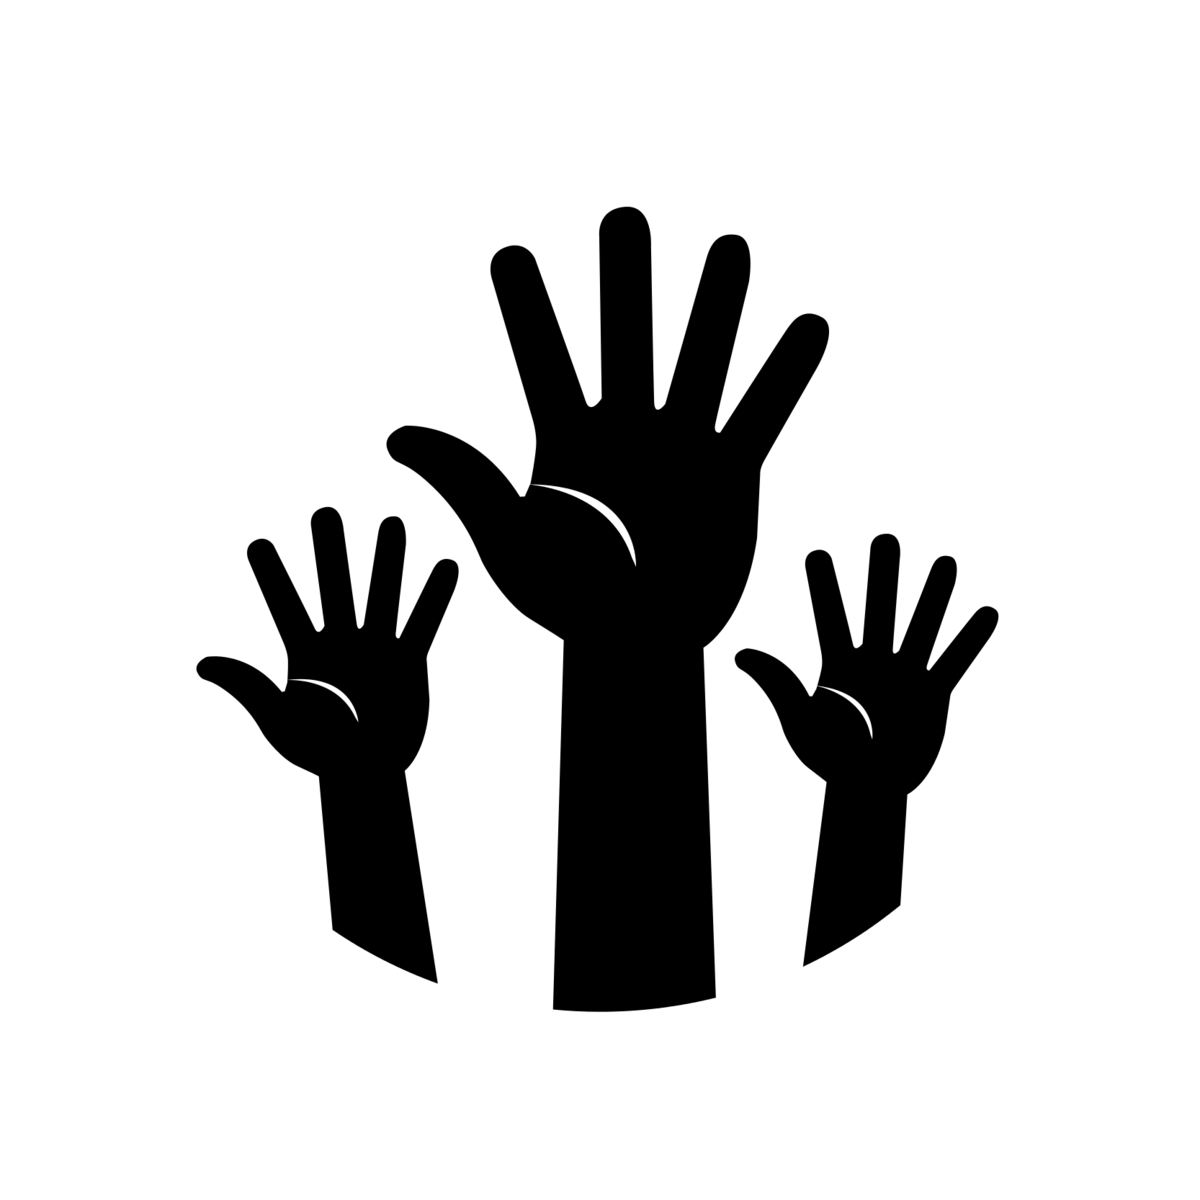
\includegraphics[scale=.1]{images/hands.png}

\end{frame}
%-----------------------------------------------------------------------
%----------------------------------------------------------------------
\begin{frame}[c]{Local Search: Uninformed random walk for SAT}

\begin{block}{SAT}
Boolean satisfiability (SAT) instances are encoded as\\ conjunctions of disjunctions of Boolean variables:

$(x_1 \vee x_2)\wedge (x_2 \vee x_3 \vee \neg x_4) \wedge (\neg x_1 \vee x_4) \wedge (\neg x_2 \vee \neg x_3)$
\end{block}

\pause

{\footnotesize
\begin{tabbing}
----\=----\=----\=----\=----\=----\=----\=----\=\kill
\pscProc\ {\em URW-for-SAT$(F,\mbox{\emph{maxSteps}})$}\\
\> {\bf input:} {\em propositional formula} $F$, \emph{integer} \emph{maxSteps}\\
\> {\bf output:} {\em model of $F$} {\bf or} $\emptyset$\\[1mm]
\onslide<2->
\> choose assignment $a$ of $F$ uniformly at random;\\
\> \emph{steps} := 0; \\
\onslide<3->
\> \pscWhile\ \pscNot(($a$ satisfies $F$)) \pscAnd{}
         (\emph{steps} $<$ \emph{maxSteps}) \pscDo\\
\onslide<4->         
\> \> randomly select variable $x$ in $F$;\\ 
\> \> change value of $x$ in $a$;\\ 
\> \> \emph{steps} := \emph{steps}$+1$;\\
\onslide<5->
\> \> \pscIf\ $a$ satisfies $F$ \pscThen \\
\> \> \> \pscReturn\ $a$\\
\> \pscEnd\\
\onslide<6->
\> \pscReturn\ $\emptyset$\\
\pscEnd\ {\em URW-for-SAT}
\end{tabbing}
}
\end{frame}
%-----------------------------------------------------------------------
%----------------------------------------------------------------------
\begin{frame}[c]{Example: URW for SAT}

\centering

$F:= (\neg x_1 \vee x_2) 
		\wedge (\neg x_2 \vee x_1) 
		\wedge (\neg x_1 \vee \neg x_2 \vee \neg x_3) 
		\wedge ( x_1 \vee x_2) 
		\wedge (\neg x_4 \vee x_3) 
		\wedge(\neg x_5 \vee x_3) 
$

\bigskip

\begin{tabular}{lccccc}
Step & $x_1$ & $x_2$ & $x_3$ & $x_4$ & $x_5$ \\ 
\hline
1 & $\top$ & $\top$ & $\top$ & $\top$ & $\top$ \\
\pause
2 & $\bot$ & $\top$ & $\top$ & $\top$ & $\top$ \\
\pause
3 & $\bot$ & $\top$ & $\bot$ & $\top$ & $\top$ \\
\pause
4 & $\bot$ & $\top$ & $\bot$ & $\top$ & $\bot$ \\
\pause
5 & $\bot$ & $\top$ & $\bot$ & $\top$ & $\top$ \\
\pause
6 & $\bot$ & $\top$ & $\bot$ & $\bot$ & $\top$ \\
\pause
7 & $\bot$ & $\top$ & $\bot$ & $\bot$ & $\bot$ \\
\pause
8 & $\top$ & $\top$ & $\bot$ & $\bot$ & $\bot$ \\
\end{tabular}

\end{frame}
%-----------------------------------------------------------------------
%----------------------------------------------------------------------
% \begin{frame}[c]{URW for SAT}
% 
% \begin{itemize}
% \item {\bf search space $S$:} set of all truth assignments to variables \\
%                 in given formula $F$
% 
% \medskip
% 
% \item {\bf solution set $S'$:} set of all models of $F$
% 
% \medskip
% 
% \onslide<2->
% \item {\bf neighbourhood relation $N$:} \emph{1-flip neighbourhood},
%         \ie{}, assignments are neighbours under $N$     iff they differ in \\
%         the truth value of exactly one variable
% 
% \bigskip
% 
% \onslide<3->
% \item {\bf memory:} not used, \ie{}, $M := \{0\}$
% \end{itemize}
% 
% \end{frame}
% %-----------------------------------------------------------------------
% %----------------------------------------------------------------------
% \begin{frame}[c]{URW for SAT}
% 
% \begin{itemize}
% \item {\bf initialization:} 
%         uniform random choice from $S$, 
%         \ie{}, $\func{init}(): (a',m) := 1/\#S$ for all assignments $a'$ and \\
%                 memory states $m$
% 
% \medskip
% 
% \onslide<2->
% \item {\bf step function:} uniform random choice from current neighbourhood,
%   \ie{}, $\func{step}(a,m): (a',m) := 1/\#N(a)$ \\
%     for all assignments $a$ and memory states $m$, \\
%     where $N(a) := \{a' \in S \mid N(a,a')\}$ is the set of \\
%     all neighbours of $a$.
% 
% \medskip
% 
% \onslide<3->
% \item {\bf termination:} when model is found, \ie{}, \\
%         $\func{terminate}(a,m):(\top) := 1$ if $a$ is a model of $F$,
%                 and $0$ otherwise.
% \end{itemize}
% 
% \end{frame}
%-----------------------------------------------------------------------
%-----------------------------------------------------------------------
\begin{frame}[c]{Improvements of URW?}

{\footnotesize
\begin{tabbing}
----\=----\=----\=----\=----\=----\=----\=----\=\kill
\pscProc\ {\em URW-for-SAT$(F,\mbox{\emph{maxSteps}})$}\\
\> {\bf input:} {\em propositional formula} $F$, \emph{integer} \emph{maxSteps}\\
\> {\bf output:} {\em model of $F$} {\bf or} $\emptyset$\\[1mm]
\> choose assignment $a$ of $F$ uniformly at random;\\
\> \emph{steps} := 0; \\
\> \pscWhile\ \pscNot(($a$ satisfies $F$) \pscAnd{}
         (\emph{steps} $<$ \emph{maxSteps})) \pscDo\\
\> \> randomly select variable $x$ in $F$;\\ 
\> \> change value of $x$ in $a$;\\ 
\> \> \emph{steps} := \emph{steps}$+1$;\\
\> \> \pscIf\ $a$ satisfies $F$ \pscThen \\
\> \> \> \pscReturn\ $a$\\
\> \pscEnd\\
\> \pscReturn\ $\emptyset$\\
\pscEnd\ {\em URW-for-SAT}
\end{tabbing}
}

\centering
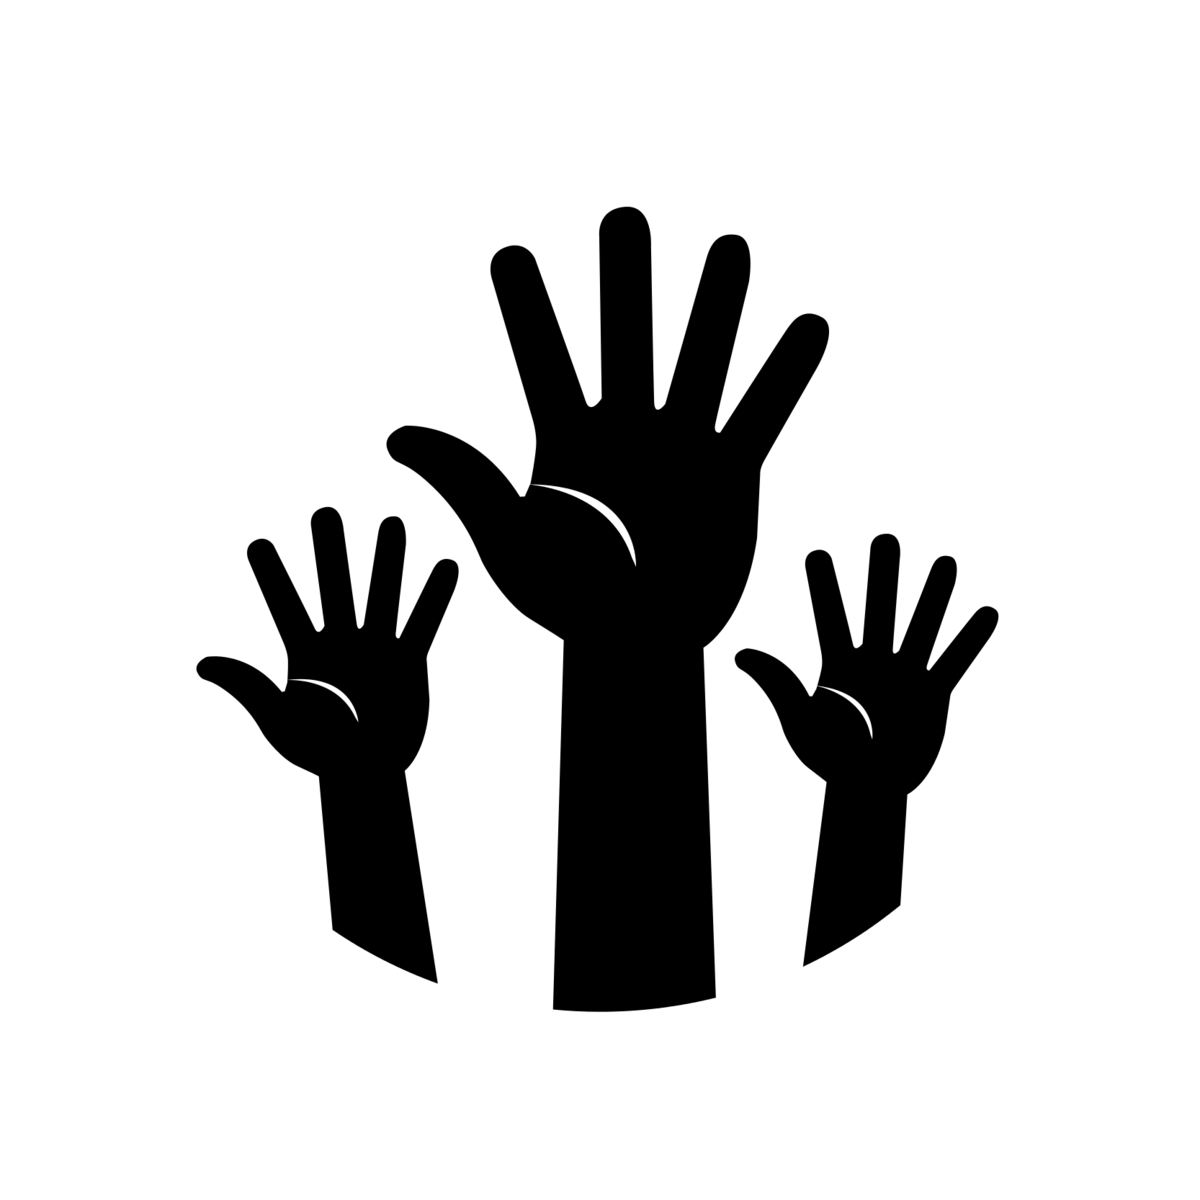
\includegraphics[scale=.05]{images/hands.png}

\end{frame}
%-----------------------------------------------------------------------
%-----------------------------------------------------------------------%-----------------------------------------------------------------------
\begin{frame}[c]{Evaluation function}

\onslide<+->
\begin{block}{Evaluation function:}
\begin{itemize}
\item function $g(\pi): S(\pi) \mapsto \Reals$ that maps candidate solutions of \\
        a given problem instance $\pi$ onto real numbers, \\
        such that global optima correspond to solutions of $\pi$;
\onslide<+->
\item used for ranking or assessing neighbours of current \\
        search position to provide guidance to search process.
\end{itemize}
\end{block}

\medskip

\onslide<+->
\begin{block}{Evaluation \vs{} objective functions:}
\begin{itemize}
\item \emph{Evaluation function}: part of SLS algorithm.
\item \emph{Objective function}: integral part of optimization problem.
\onslide<+->
\item Some SLS methods use evaluation functions different from
        given objective function (\eg{}, dynamic local search).
\end{itemize}
\end{block}

\end{frame}
%-----------------------------------------------------------------------
% %-----------------------------------------------------------------------
% \begin{frame}[c]{Iterative Improvement (II)}
% 
% \onslide<+->
% \begin{itemize}
% \item does not use memory
% \item $\func{init}$: uniform random choice from $S$
% 
% \onslide<+->
% \item $\func{step}$: uniform random choice from improving neighbours, \\
%         \ie{}, $\func{step}(s): (s') := 1/\#I(s)$ if $s' \in I(s)$,
%         and $0$ otherwise, \\
%         where $I(s) := \{s' \in S \mid N(s,s') \wedge g(s') < g(s)\}$
% 
% \medskip
%         \onslide<+->
% \item terminates when no improving neighbour available\\
%         (to be revisited later)
% \medskip
%         \onslide<+->
% \item different variants through modifications of step function\\
%         (to be revisited later)
% 
% \end{itemize}
% 
% \medskip
% 
% \onslide<+->
% \emph{Note:} II is also known as \emph{iterative descent}
%         or \emph{hill-climbing}.
% 
% \end{frame}
% %-----------------------------------------------------------------------
% %-----------------------------------------------------------------------
% \begin{frame}[c]{Iterative Improvement for SAT}
% 
% 
% \begin{itemize}
% \item {\bf search space $S$:} set of all truth assignments to variables \\
%                 in given formula $F$
% \item {\bf solution set $S'$:} set of all models of $F$
% \item {\bf neighbourhood relation $N$:} 1-flip neighbourhood \\
%         (as in Uninformed Random Walk for SAT)
% 
% \medskip
% 
% \onslide<+->
% \item {\bf memory:} not used, \ie{}, $M := \{0\}$
% 
% \item {\bf initialization:} 
%         uniform random choice from $S$, 
%         \ie{}, $\func{init}() : (a',m) := 1/\#S$ for all assignments $a'$\\
%         and memory states $m$
% 
% \end{itemize}
% 
% \end{frame}
% %-----------------------------------------------------------------------
% %-----------------------------------------------------------------------
% \begin{frame}[c]{Iterative Improvement for SAT}
% 
% \begin{itemize}
% \item {\alert
%         {\bf evaluation function:} $g(a) := $ number of clauses in $F$ \\
%         that are \emph{unsatisfied} under assignment $a$\\
%         }
%         (\emph{Note:} $g(a)=0$ iff $a$ is a model of $F$.)
%   
% 
% \medskip
% 
% \onslide<+->
% \item {\bf step function}: uniform random choice from improving neighbours,
%         \ie{}, $\func{step}(a)(a') := 1/\#I(a)$ if $s' \in I(a)$, \\
%         and $0$ otherwise,
%         where $I(a) := \{a' \mid N(a,a') \wedge g(a') < g(a)\}$
% 
% \medskip
% 
% \onslide<+->
% \item {\bf termination}: when no improving neighbour is available \\
%         \ie{}, $\func{terminate}(a)(\top):=1$ if $I(a)=\emptyset{}$,
%                 and $0$ otherwise.
% \end{itemize}
% 
% \onslide<+->
% \medskip
% \alert{Problem}: II will get stuck in local minima.
% 
% \end{frame}
% %-----------------------------------------------------------------------
%----------------------------------------------------------------------
\begin{frame}[c]{Iterative Improvement with Local Search: WalkSAT\\ \litw{B. Selman et al. 2006}}

\smallskip
{\footnotesize
\begin{tabbing}
----\=----\=----\=----\=----\=----\=----\=----\=\kill
\pscProc\ {\em WalkSAT$(F,\mbox{\emph{maxSteps}})$}\\
\> {\bf input:} {\em propositional formula} $F$, \emph{integer} \emph{maxSteps}\\
\> {\bf output:} {\em model of $F$} {\bf or} $\emptyset$\\[1mm]
\> choose assignment $a$ of $F$ uniformly at random;\\
\> \pscIf\ $a$ satisfies $F$ \textbf{then return} $a$\\
\> \emph{steps} := 0; \\
\> \pscWhile\ (\emph{steps} $<$ \emph{maxSteps}) \pscDo\\
\> \> randomly select an unsatisfied clause $C$;\\ 
\> \> randomly select a variable $v$ that appears in $C$;\\ 
\> \> change the value of $v$ and keep the change unless it\\
\> \> increases the number of unsatisfied clauses;\\ 
%\> \> randomly select variable $x$ in $F$;\\ 
%\> \> change value of $x$ in $a$;\\ 
\> \> \emph{steps} := \emph{steps}$+1$;\\
\> \> \pscIf\ $a$ satisfies $F$ \textbf{then return} $a$\\
\> \pscEnd\\
\> \pscReturn\ $\emptyset$\\
\pscEnd\ {\em WalkSAT}
\end{tabbing}
}
\end{frame}
%-----------------------------------------------------------------------
%----------------------------------------------------------------------
\begin{frame}[c]{Example: WalkSAT for SAT}

\centering

$F:= (\neg x_1 \vee x_2) 
		\wedge (\neg x_2 \vee x_1) 
		\wedge (\neg x_1 \vee \neg x_2 \vee \neg x_3) 
		\wedge ( x_1 \vee x_2) 
		\wedge (\neg x_4 \vee x_3) 
		\wedge(\neg x_5 \vee x_3) 
$

\bigskip

\begin{tabular}{lcccccc}
Step & $x_1$ & $x_2$ & $x_3$ & $x_4$ & $x_5$ & Confl. Clauses\\ 
\hline
1 & $\top$ & $\top$ & $\bot$ & $\top$ & $\top$ & $C_5,C_6$\\
\pause
2 & $\top$ & $\top$ & $\bot$ & $\top$ & $\bot$ & $C_5$\\
\pause
3 & $\top$ & $\top$ & $\top$ & $\top$ & $\bot$ & $C_3$ $\to$ rejected\\
\pause
4 & $\top$ & $\top$ & $\bot$ & $\bot$ & $\bot$ & $\checkmark$\\
\end{tabular}

\end{frame}
%-----------------------------------------------------------------------
% %-----------------------------------------------------------------------
% \begin{frame}[c]{Global vs. Local Optima}
% 
% \onslide<+->
% \begin{block}{Global Optima}
% A global optimum is a search position $s$ with the optimal value of $g(s)$ in the entire search space.
% \end{block}
% 
% \medskip
% 
% \onslide<+->
% \begin{block}{Local Optima}
% A local optima is a search position $s$ with the best value of $g(s)$ in the neighbourhood of $s$.
% \end{block}
% 
% \medskip
% 
% \onslide<+->
% \begin{block}{Plateau}
% Plateaus is a region of search positions with identical evaluation function values.
% \end{block}
% 
% \end{frame}
% %-----------------------------------------------------------------------
% %-----------------------------------------------------------------------
% \begin{frame}{Global vs. Local Optima}
% 
% Extra Space for diagram 
% 
% \end{frame}
% %-----------------------------------------------------------------------
%-----------------------------------------------------------------------
\begin{frame}[c]{Escaping from local optima}

\onslide<+->
\begin{itemize}
\item \emph{Restart:} re-initialize search\\ whenever a local optimum 
        is encountered.\\
         (Sometimes rather ineffective due to cost of initialization.)

\medskip

\onslide<+->
\item \emph{Non-improving steps}:  allow selection of \\
        candidate solutions with equal or worse evaluation function value,
        \eg{}, using minimally worsening steps.\\
        (Can lead to long walks in \emph{plateaus}.)
        
\end{itemize}

\bigskip

\onslide<+->
\emph{Note:} None of these mechanisms is guaranteed to always \\
        effectively escape from local optima.
        
\end{frame}
%-----------------------------------------------------------------------
% %-----------------------------------------------------------------------
% \begin{frame}[c, fragile]{Task: Improved SLS Algorithms}
% 
% \begin{columns}
% \column{0.6\textwidth}
% 
% \includegraphics[scale=0.3]{images/uncle_sam}
% 
% \begin{enumerate}
%   \item each group (at most 3 students) one algorithm
%   \item 10 minutes for understanding
%   \item each group presents the algorithm
%   \item application of algorithm to SAT?
% \end{enumerate}
% 
% \column{0.4\textwidth}
% 
% Algorithms: 
% 
% \begin{enumerate}
%   \item Randomized Iterative Improvement,
%   \item Variable Neighbourhood Descent, 
%   \item Simulated Annealing,
%   \item Tabu Search,
%   \item Dynamic Local Search,
%   \item Iterated Local Search,
%   \item Greedy Randomized ``Adaptive'' Search Procedure
% \end{enumerate}
% 
% \end{columns}
% 
% 
% \end{frame}
% %-----------------------------------------------------------------------
%-----------------------------------------------------------------------
\begin{frame}[c]{Randomized Iterative Improvement (RII)}

\begin{tabbing}
----\=----\=----\=----\=----\=----\=----\=----\=\kill
\> determine initial candidate solution $s$\\
\> \pscWhile\ termination condition is not satisfied:\\
\> \vbar \> With probability \param{wp}:\\[-0.55ex]
\> \vbar \> \>  choose a neighbour $s'$ of $s$ uniformly at random\\[-0.55ex]
\> \vbar \> Otherwise:\\[-0.55ex]
\> \vbar \> \>  choose a neighbour $s'$ of $s$ such that $g(s') < g(s)$ or,\\[-0.55ex]
\> \vbar \> \>  \hspace*{0.4em} if no such $s'$ exists, 
                                                                choose $s'$ such that $g(s')$ is minimal\\[-0.55ex]
\> \vend \> $s$ := $s'$
\end{tabbing}

\pause

\medskip
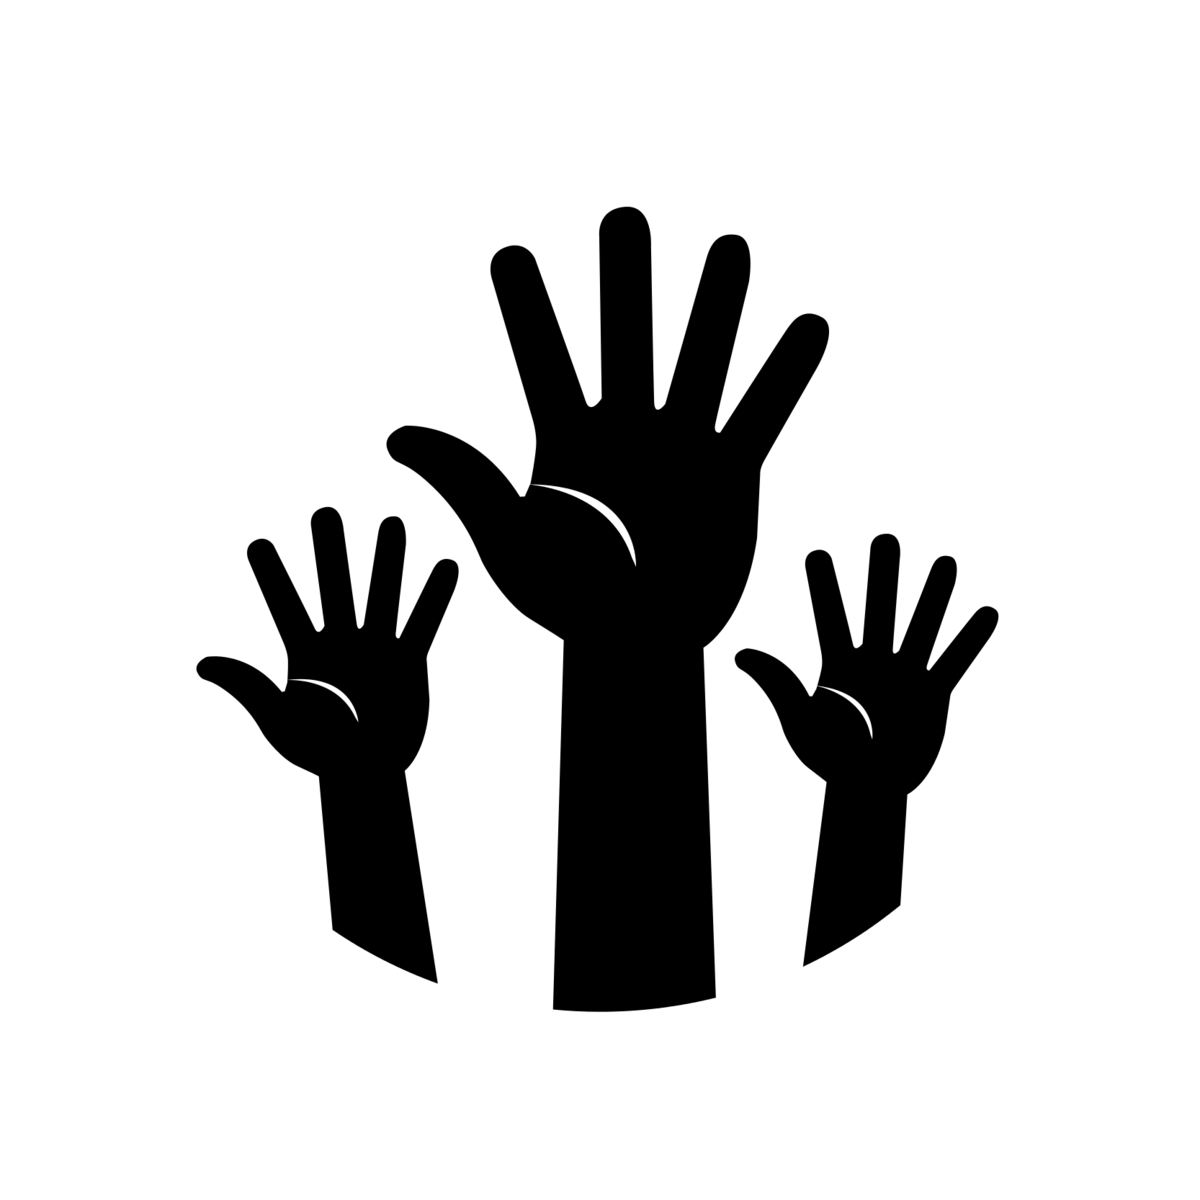
\includegraphics[scale=.03]{images/hands.png}
\alert{Design decisions?}:\\
\pause Probability parameter wp, evaluation function~$g$,\\ construction method of initial candidate

\end{frame}
%-----------------------------------------------------------------------
%----------------------------------------------------------------------
\begin{frame}[c]{Example: RII for SAT}

\centering

$F:= (\neg x_1 \vee x_2) 
		\wedge (\neg x_2 \vee x_1) 
		\wedge (\neg x_1 \vee \neg x_2 \vee \neg x_3) 
		\wedge ( x_1 \vee x_2) 
		\wedge (\neg x_4 \vee x_3) 
		\wedge(\neg x_5 \vee x_3) 
$

\bigskip

\begin{tabular}{lccccccc}
Step. & $x_1$ & $x_2$ & $x_3$ & $x_4$ & $x_5$ & Confl. Clauses & $g(s)$\\ 
\hline
1 Init & $\top$ & $\top$ & $\top$ & $\top$ & $\top$ & $C_3$ & $1$\\
\pause
2 Non-Impr. & $\top$ & $\top$ & $\bot$ & $\top$ & $\top$ & $C_5,C_6$ & $2$\\
\pause
3 Random & $\top$ & $\bot$ & $\bot$ & $\top$ & $\top$ & $C_1,C_4,C_5,C_6$ & $4$\\
\pause
4 Impr. & $\top$ & $\bot$ & $\bot$ & $\bot$ & $\top$ & $C_1,C_4,C_6$ & $3$\\
\pause
5 Impr. & $\top$ & $\bot$ & $\bot$ & $\bot$ & $\bot$ & $C_1,C_4$ & $2$\\
\pause
6 Random & $\top$ & $\bot$ & $\top$ & $\bot$ & $\bot$ & $C_1,C_4$ & $2$\\
\pause
7 Impr. & $\top$ & $\top$ & $\top$ & $\bot$ & $\bot$ & $C_3$ & $1$\\
\pause
8 Impr. & $\top$ & $\top$ & $\bot$ & $\bot$ & $\bot$ & $\checkmark$ & $0$\\
\end{tabular}

\end{frame}
%-----------------------------------------------------------------------
%-----------------------------------------------------------------------
\begin{frame}[c]{Variable Neighbourhood Descent (VND)}

\begin{block}{Idea}
Change (typically increase) the size of the neighbourhood relation over time. 
%I.e., $N_1,\ldots,N_{imax}$ is a set of neighbourhood relations, 
%typically ordered according to increasing size of the respective local neighbourhoods.
\end{block}

\begin{tabbing}
----\=----\=----\=----\=----\=----\=----\=----\=\kill
\> determine initial candidate solution $s$\\
\> $i$ := $1$\\
\> \pscRepeat\\
\> \vbar \> choose most improving neighbour $s'$ of $s$ in $N_i$\\[-0.55ex]
\> \vbar \> \pscIf\ $g(s') < g(s)$:\\[-0.55ex]
\> \vbar \> \> $s$ := $s'$\\[-0.55ex]
\> \vbar \> \> $i$ := $1$\\[-0.55ex]
\> \vbar \> \pscElse\ \\[-0.55ex]
\> \vendbar \> \> $i$ := $i+1$\\[-0.55ex]
\> \pscUntil\ $i > \param{k}$
\end{tabbing}

\pause

\vspace{-0.5cm}
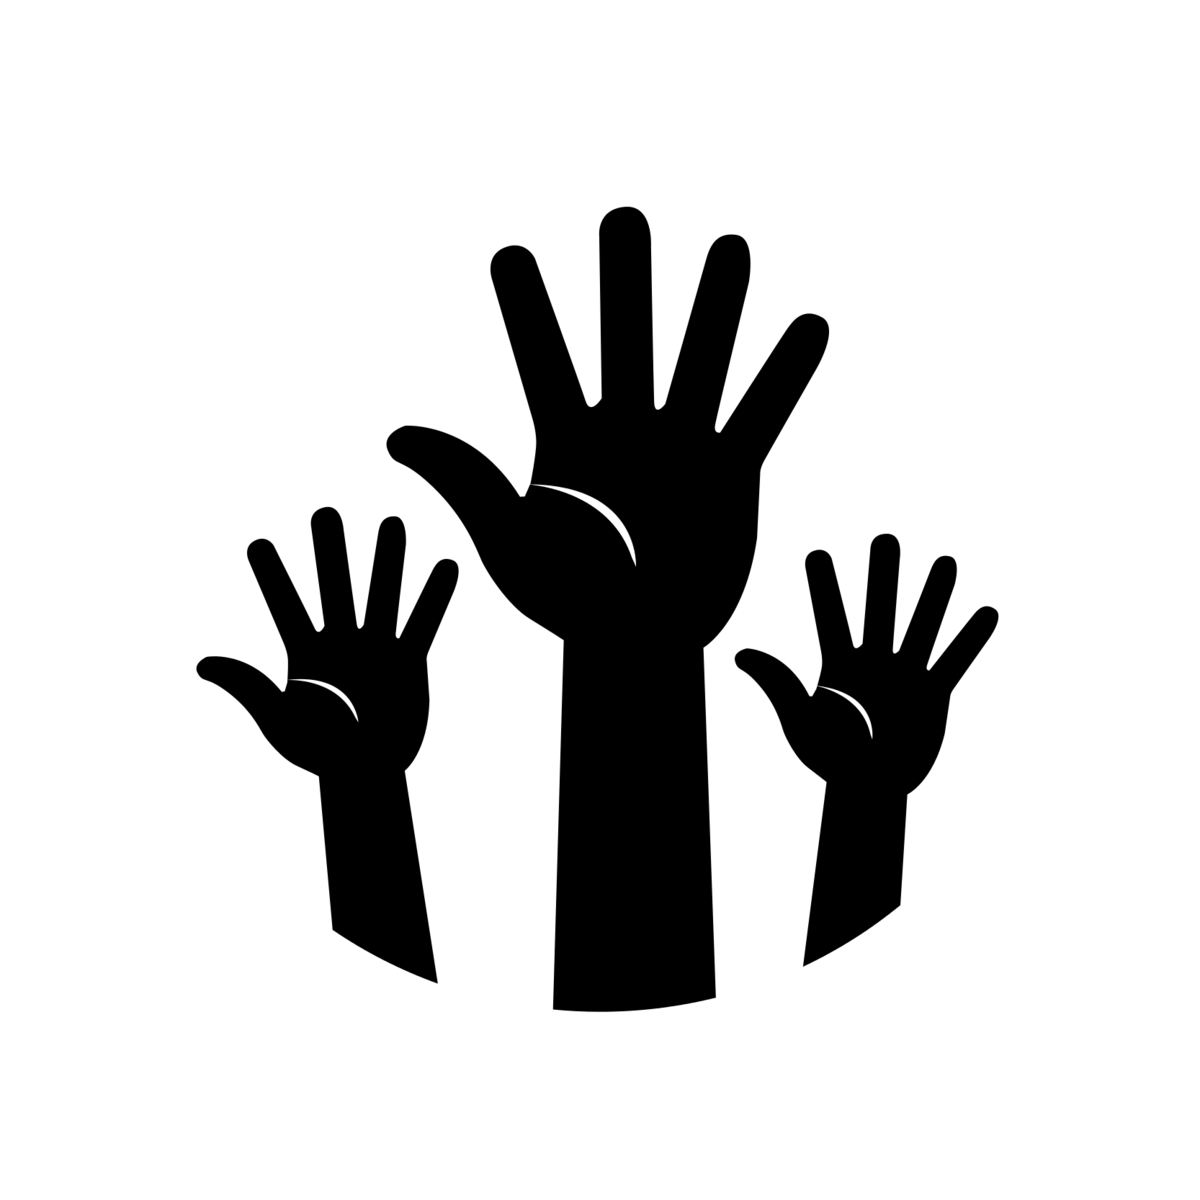
\includegraphics[scale=.03]{images/hands.png}
\alert{Design decisions?}:
\pause Design of increasing neighbourhood relation, evaluation function $g$,
construction method of initial candidate

\end{frame}
%-----------------------------------------------------------------------
%----------------------------------------------------------------------
\begin{frame}[c]{Example: VND for SAT}

\centering

$F:= (\neg x_1 \vee x_2) 
		\wedge (\neg x_2 \vee x_1) 
		\wedge (\neg x_1 \vee \neg x_2 \vee \neg x_3) 
		\wedge ( x_1 \vee x_2) 
		\wedge (\neg x_4 \vee x_3) 
		\wedge(\neg x_5 \vee x_3) 
$

\bigskip

\begin{tabular}{lccccccc}
Step. & $x_1$ & $x_2$ & $x_3$ & $x_4$ & $x_5$ & Confl. Clauses & $g(s)$\\ 
\hline
1 Init $i=1$ & $\top$ & $\top$ & $\top$ & $\top$ & $\top$ & $C_3$ & $1$\\
\pause
2 No Impr. $i=2$ & $\top$ & $\top$ & $\top$ & $\top$ & $\top$ & $C_3$ & $1$\\
\pause
3 No Impr. $i=3$ & $\top$ & $\top$ & $\top$ & $\top$ & $\top$ & $C_3$ & $1$\\
\pause
4 Impr. $i=1$ & $\top$ & $\top$ & $\bot$ & $\bot$ & $\bot$ & $\checkmark$ & $0$\\
\end{tabular}

\bigskip
\pause

Note: With large neighborhoods sizes, you have to check more potential solution candidates
to find the most improving neighbour. 

\end{frame}
%-----------------------------------------------------------------------
%-----------------------------------------------------------------------
\begin{frame}[c]{Simulated Annealing (SA)}

\begin{tabbing}
----\=----\=----\=----\=----\=----\=----\=----\=\kill
\> determine initial candidate solution $s$\\
\> set initial temperature $T$ according to annealing schedule\\
\> \pscWhile\ termination condition is not satisfied:\\
\> \vbar \> probabilistically choose a neighbour $s'$ of $s$ \\[-0.55ex]
\> \vbar \> \> using proposal mechanism\\[-0.55ex] 
\> \vbar \> \pscIf\ $s'$ satisfies probabilistic acceptance criterion ($p_{accept}(T,s,s')$):\\[-0.55ex]
\> \vbar \> \> $s$ := $s'$\\[-0.55ex]
\> \vend \> update $T$ according to annealing schedule
\end{tabbing}

\begin{equation}
p_{accept}(T,s,s')= \begin{cases}
					1 & \text{if } g(s') \leq g(s)\\
					\exp\left(\frac{g(s)-g(s')}{T}\right)  & \text{otherwise}
\end{cases}\nonumber
\end{equation}

\pause

Note: The annealing schedule may keep $T$ constant for a number of search steps.

\medskip
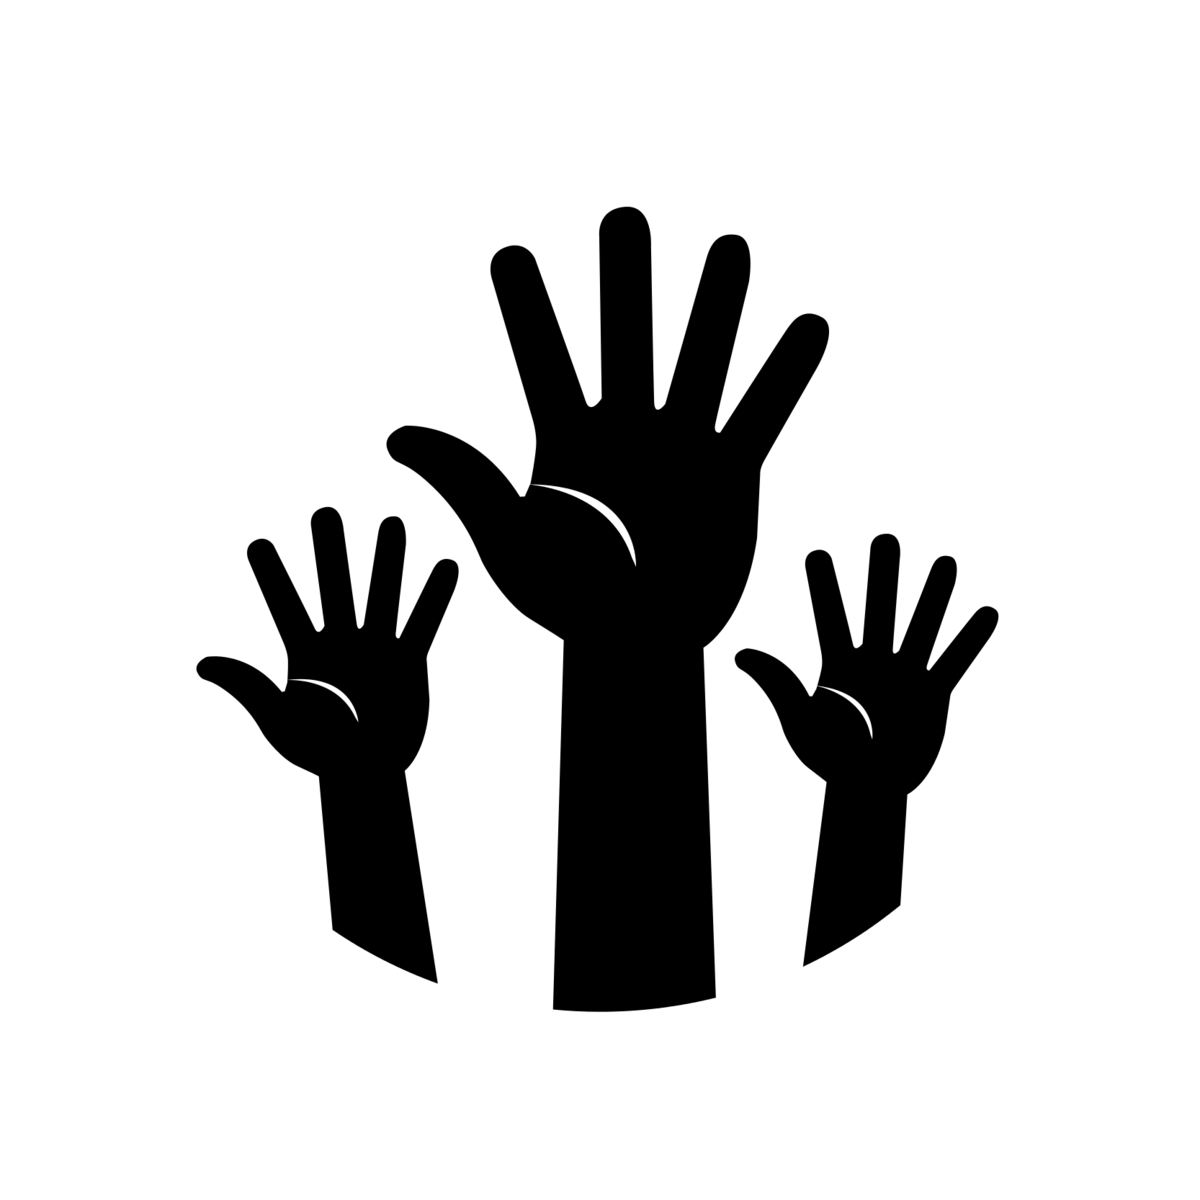
\includegraphics[scale=.01]{images/hands.png}
\alert{Design decisions?}:\\
\pause annealing schedule, proposal mechanism,\\ 
construction method of initial candidate

\end{frame}
%-----------------------------------------------------------------------
%-----------------------------------------------------------------------
\begin{frame}[c]{Tabu Search}

\begin{tabbing}
----\=----\=----\=----\=----\=----\=----\=----\=\kill
\> determine initial candidate solution $s$\\
\> \pscWhile\ \emph{termination criterion} is not satisfied:\\
\> \vbar \> determine set $N'$ of non-tabu neighbours of $s$\\[-0.55ex]
\> \vbar \> choose a best improving candidate solution $s'$ in $N'$\\[-0.55ex]
\> \vbar \\[-1.5ex]
\> \vbar \> update tabu attributes based on $s'$\\[-0.55ex]
\> \vend \> $s$ := $s'$ 
\end{tabbing}

Note: Tabu attributes are associated with solution components.

\medskip
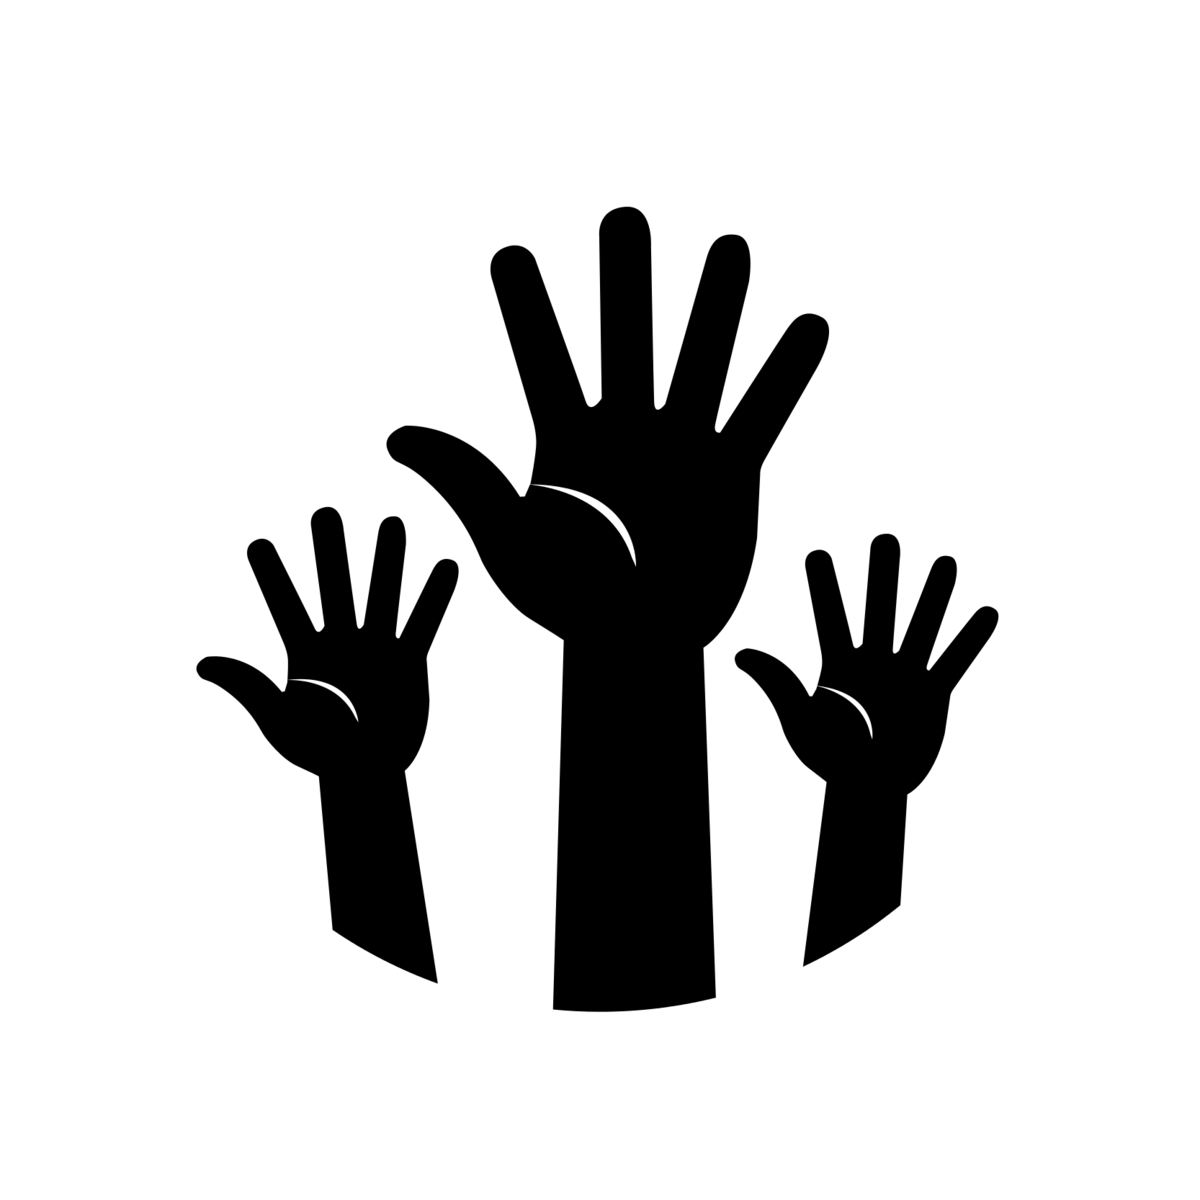
\includegraphics[scale=.03]{images/hands.png}
\alert{Design decisions?}:\\
\pause Design of tabu mechanism,\\ 
construction method of initial candidate

\end{frame}
%-----------------------------------------------------------------------
%----------------------------------------------------------------------
\begin{frame}[c]{Example: Tabu-Search for SAT}

\centering

$F:= (\neg x_1 \vee x_2) 
		\wedge (\neg x_2 \vee x_1) 
		\wedge (\neg x_1 \vee \neg x_2 \vee \neg x_3) 
		\wedge ( x_1 \vee x_2) 
		\wedge (\neg x_4 \vee x_3) 
		\wedge(\neg x_5 \vee x_3) 
$

\bigskip

\begin{tabular}{lccccccc}
Step. & $x_1$ & $x_2$ & $x_3$ & $x_4$ & $x_5$ & Confl. Clauses & Tabu\\ 
\hline
1 & $\bot$ & $\bot$ & $\bot$ & $\bot$ & $\bot$ & $C_4$ & $\emptyset$\\
\pause
2 & $\top$ & $\bot$ & $\bot$ & $\bot$ & $\bot$ & $C_1$ & $\{x_1\}$\\
\pause
3 & $\top$ & $\top$ & $\bot$ & $\bot$ & $\bot$ & $\checkmark$ & $\{x_1,x_2\}$\\
\end{tabular}


\end{frame}
%-----------------------------------------------------------------------
%-----------------------------------------------------------------------
\begin{frame}[c]{Dynamic Local Search (DLS)}

\begin{tabbing}
----\=----\=----\=----\=----\=----\=----\=----\=\kill
\> determine \emph{initial candidate solution $s$}\\
\> initialize penalties\\
\> \pscWhile\ \emph{termination criterion} is not satisfied:\\
\> \vbar \> compute modified evaluation function $g'$ from $g$ \\[-0.55ex]
\> \vbar \> \>                          based on penalties\\[-0.55ex]
\> \vbar \\[-1.5ex]
\> \vbar \> perform subsidiary local search on $s$ \\[-0.55ex]
\> \vbar \> \>        using evaluation function $g'$ \\[-0.55ex]
\> \vbar \\[-1.5ex]
\> \vend \> update penalties based on $s$
\end{tabbing}

Note: Penalties are associated with solution components; 
the subsidiary local search ends in a local optimum of $g'$.

\medskip
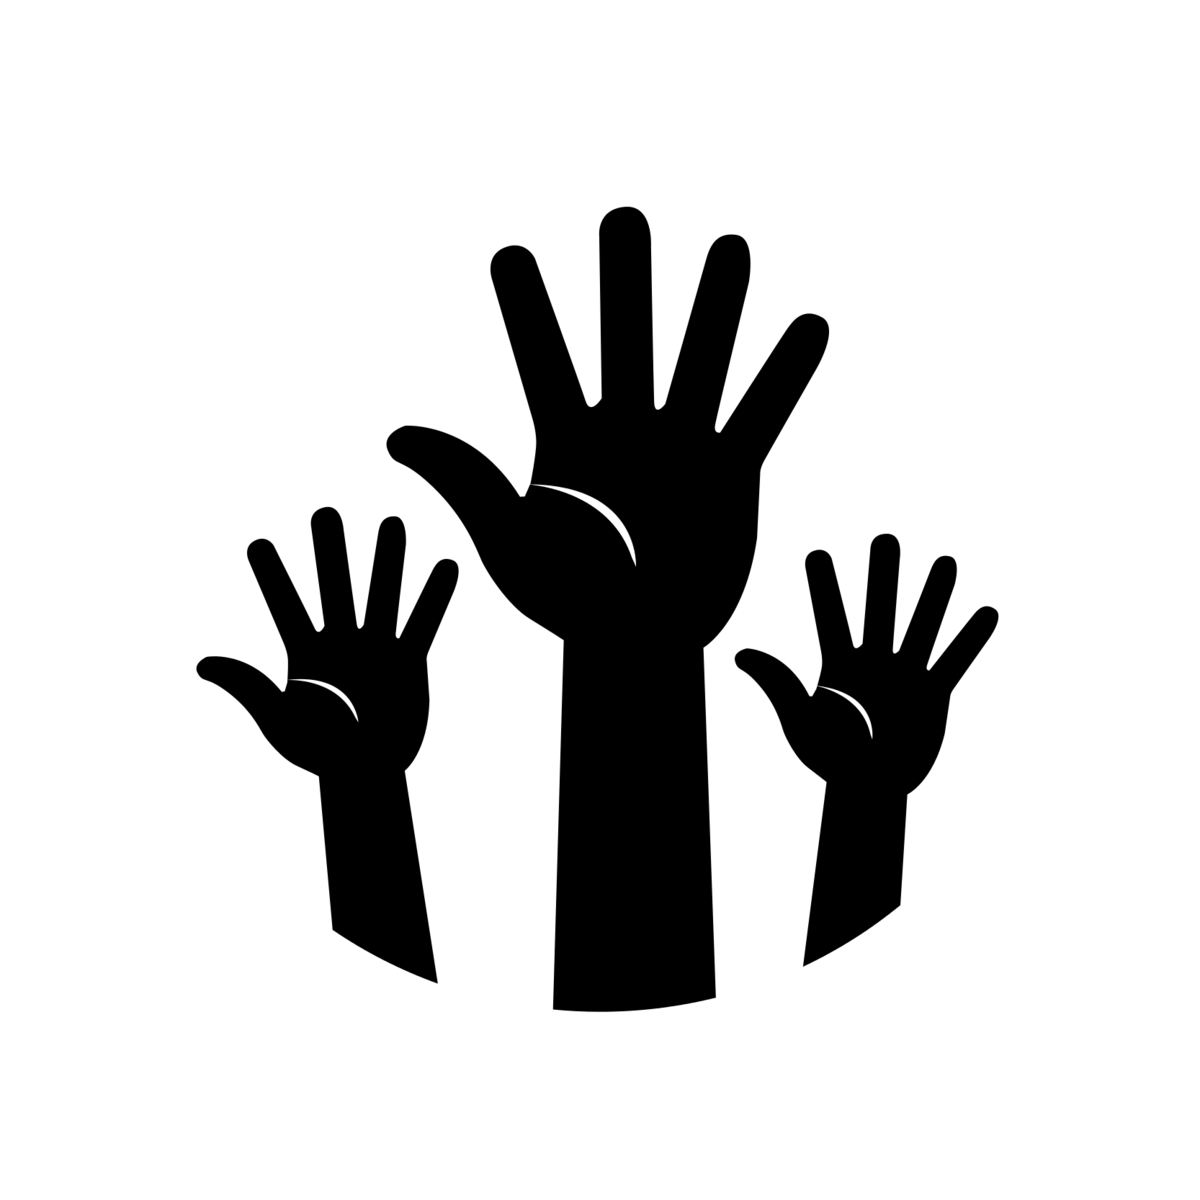
\includegraphics[scale=.03]{images/hands.png}
\alert{Design decisions?}:\\
\pause Design of $g$ (penalties), subsidiary local search \\ 
construction method of initial candidate

\end{frame}
%-----------------------------------------------------------------------
%-----------------------------------------------------------------------
\begin{frame}[c]{Iterated Local Search (ILS)}

\begin{tabbing}
----\=----\=----\=----\=----\=----\=----\=----\=\kill
\> determine initial candidate solution $s$\\
\> perform subsidiary local search on $s$\\
\> \pscWhile\ termination criterion is not satisfied:\\
\> \vbar \> $r$ := $s$\\[-0.55ex]
\> \vbar \> perform perturbation on $s$ \hspace{0.8em} \texttt{\% n random steps in neighbourhood}\\[-0.55ex]
\> \vbar \> perform subsidiary local search on $s$\\[-0.55ex]
\> \vbar \\[-1.5ex]
\> \vbar\> based on acceptance criterion, \\[-0.55ex]
\> \vend \> \> keep $s$ or revert to $s:=r$
\end{tabbing}

Note: The search history may additionally influence the perturbation phase
and the acceptance criterion.

\medskip
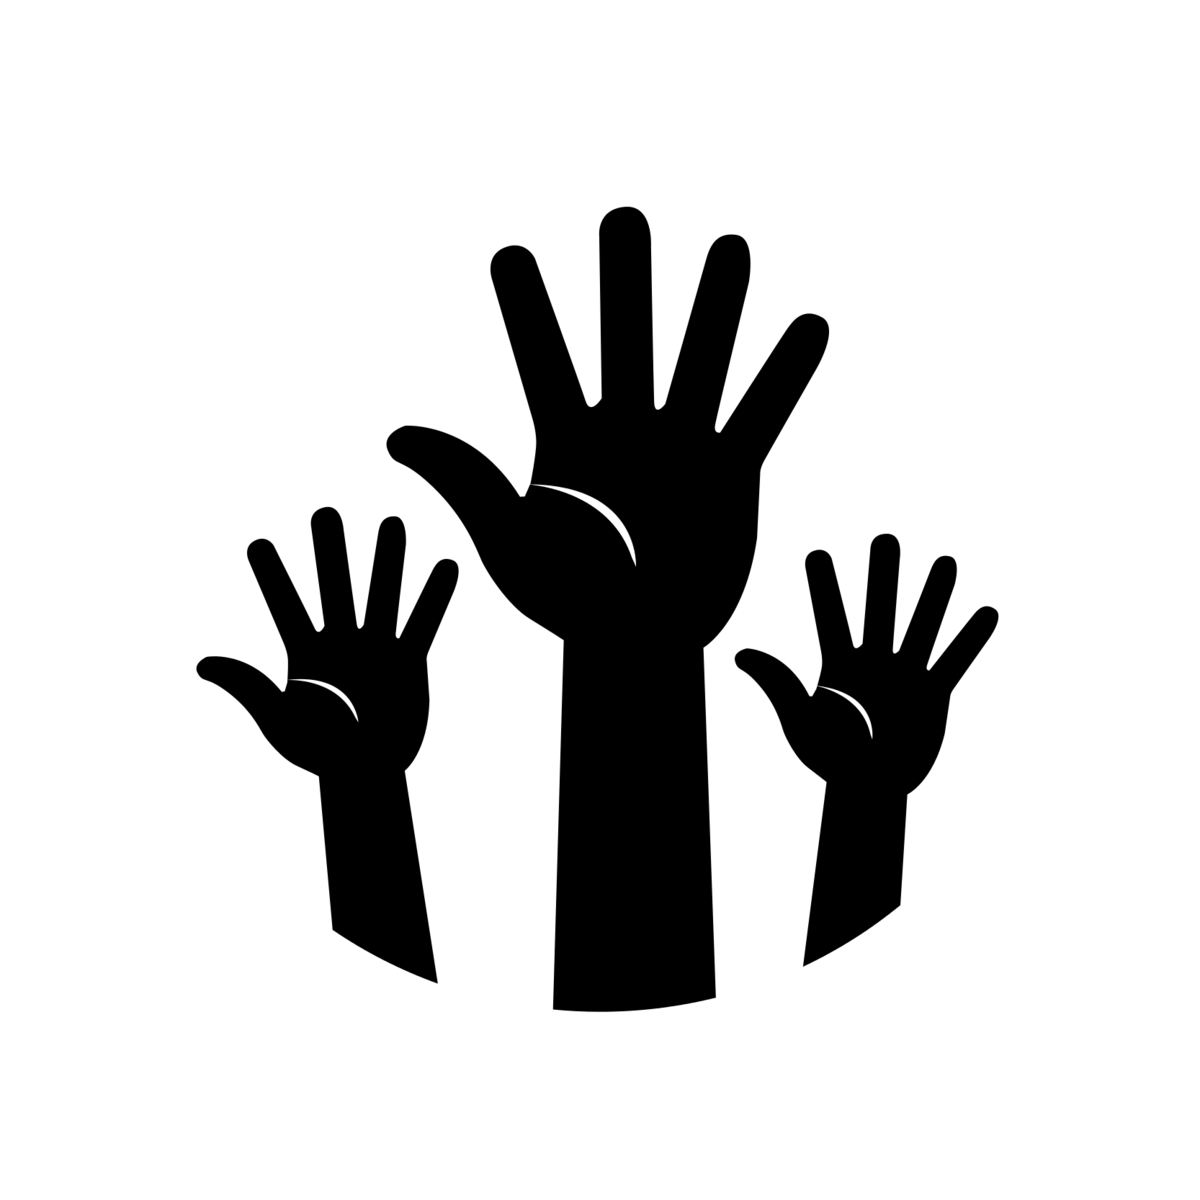
\includegraphics[scale=.03]{images/hands.png}
\alert{Design decisions?}:\\
\pause Strength of perturbation, subsidiary local search, acceptance criterion\\ 
construction method of initial candidate

\end{frame}
%-----------------------------------------------------------------------
% %-----------------------------------------------------------------------
% \begin{frame}[c]{Greedy Randomized ``Adaptive'' Search Procedure (GRASP)}
% 
% \begin{tabbing}
% ----\=----\=----\=----\=----\=----\=----\=----\=\kill
% \> \pscWhile\ \emph{termination criterion} is not satisfied:\\
% \> \vbar \> generate candidate solution $s$ using \\[-0.55ex]
% \> \vbar \> \>  subsidiary greedy randomized constructive search\\[-0.55ex]
% \> \vbar \\[-1.5ex]
% \> \vend \> perform subsidiary local search on $s$
% \end{tabbing}
% 
% Note: Randomization in \emph{constructive search} ensures that a large number
%         of good starting points for \emph{subsidiary local search} is obtained.
% 
% \begin{block}{Constructive Search:}
% \begin{enumerate}
%   \item Start with an empty candidate solution
%   \item Repeatedly, extend the current solution until a complete solution is constructed
%   \item Use heuristics to extend in such a way that the final solution is a good one
% \end{enumerate}
% \end{block}
% 
% \end{frame}
% %-----------------------------------------------------------------------
%----------------------------------------------------------------------
\begin{frame}[c]{}

\centering
\huge
Solving Combinatorial Problems:\\
Evolutionary Algorithms

\end{frame}
%----------------------------------------------------------------------
%----------------------------------------------------------------------
\begin{frame}[c]{Population-based Algorithms}

\begin{block}{Population:}
\begin{itemize}
  \item Set of candidate solutions $=$ population of individuals
  \item Evolve population over time such that ``fitness'' of population improves
  \item Fitness: can either correspond to objective function $f$ or evaluation function $g$
\end{itemize}
\end{block}

\pause

\begin{block}{Comparison to SLS:}
\begin{itemize}
  \item SLS typically converges faster to good intermediate solution
  \item Population-based algorithms are less often trapped in local optima
  \item Population-based algorithms are even easier to parallelize
  \begin{itemize}
    \item evaluate $f$ (or $g$) of each individual in parallel
  \end{itemize}
\end{itemize}
\end{block}

\end{frame}
%----------------------------------------------------------------------
%----------------------------------------------------------------------
\begin{frame}[c]{Genetic Algorithms}

\begin{center} 
	\includegraphics[width=0.50\textwidth]{images/ea.png}  
\end{center}
{\tiny Source: ``Introduction to Evoluationary Computing'' by Eiben and Smith }

\bigskip
\pause

\begin{block}{Central Idea}
A solution candidate can be described by its solution components\\ (also called genes),
for example, variable assignment of each variable.
\end{block}

\bigskip
\pause
Note: Each step of a genetic algorithm implies new design choices!

\end{frame}
%----------------------------------------------------------------------
%----------------------------------------------------------------------
\begin{frame}[c]{Genetic Algorithms: Mutation}

\begin{block}{Mutation:}
\begin{itemize}
  \item With probability $p$, mutate a given individual.
  \item Mutation: perturbate a solution candidate 
\end{itemize}
\end{block}

\pause
\bigskip

\centering
\begin{tabular}{lccccc}
& $x_1$ & $x_2$ & $x_3$ & $x_4$ & $x_5$\\
\hline
Parent & $\bot$ & $\bot$ & $\bot$ & $\bot$ & $\bot$ \\
\pause
Offspring & $\bot$ & $\top$ & $\bot$ & $\bot$ & $\bot$ \\
\end{tabular}

\pause
\medskip
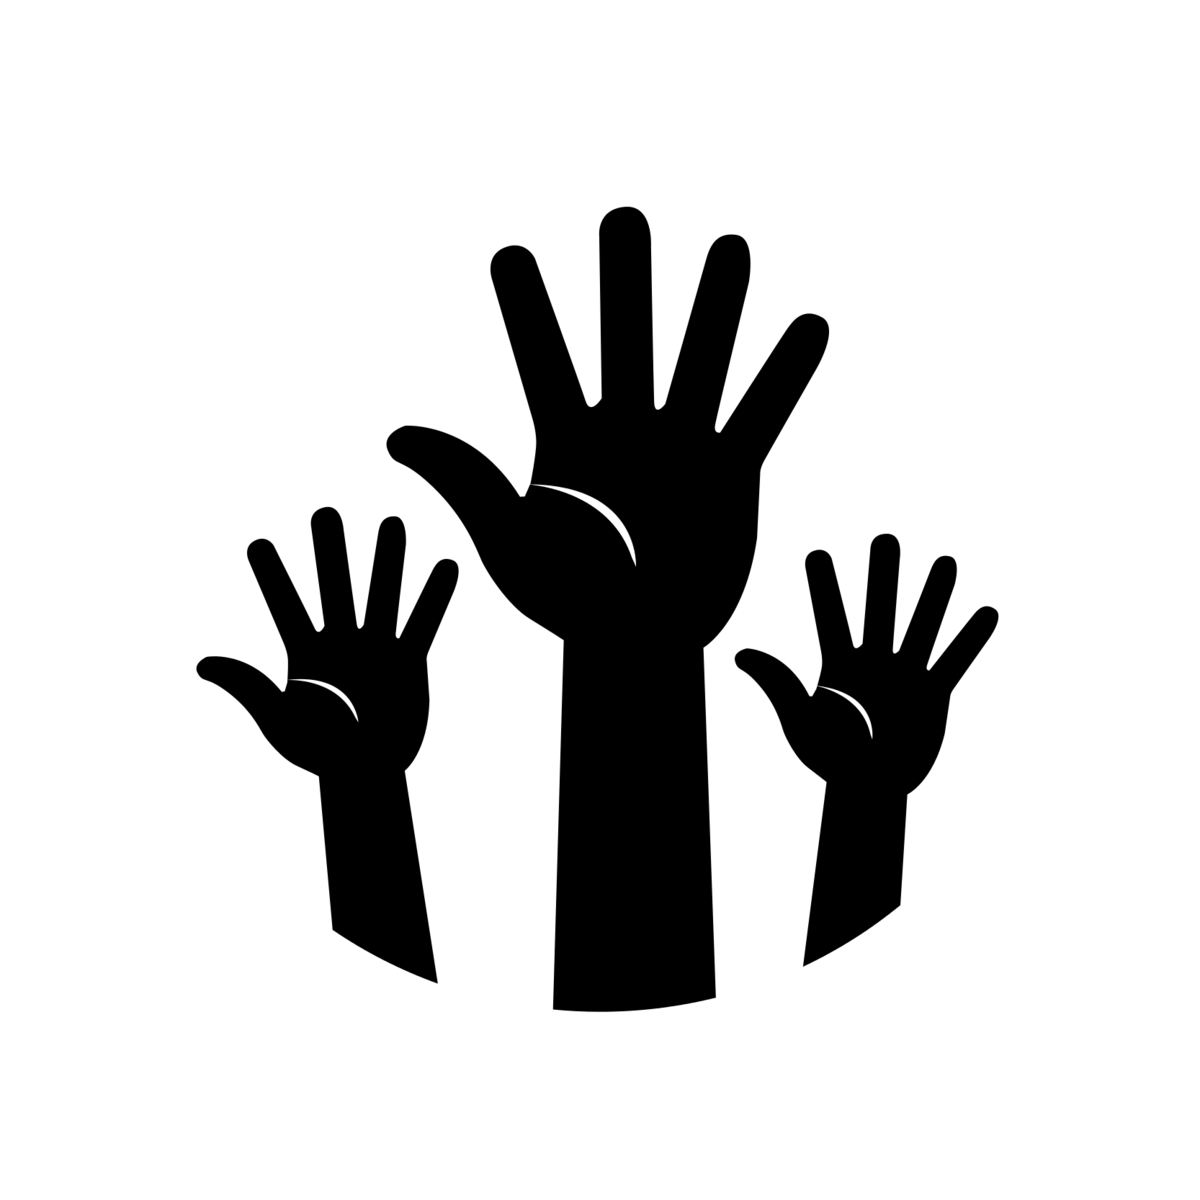
\includegraphics[scale=.03]{images/hands.png}
\alert{Design decisions?}:\\
\pause Strength of mutation, probability of mutation,\\
mutation operator (e.g., bit-wise or swaps)


\end{frame}
%----------------------------------------------------------------------
%----------------------------------------------------------------------
\begin{frame}[c]{Genetic Algorithms: Recombination}

\begin{block}{Mutation:}
\begin{itemize}
  \item Selection of two parents
  \item Recombine them to obtain off-spring
\end{itemize}
\end{block}

\pause
\bigskip

\centering
\begin{tabular}{lcccccc}
& $x_1$ & $x_2$ & & $x_3$ & $x_4$ & $x_5$\\
\hline
Parent 1 & $\bot$ & $\bot$ & & $\bot$ & $\bot$ & $\bot$ \\
Parent 2 & $\top$ & $\bot$ & & $\top$ & $\bot$ & $\top$ \\
\pause
Offspring & $\bot$ & $\bot$ & $\mid$ & $\top$ & $\bot$ & $\top$ \\
\end{tabular}

\pause
\medskip
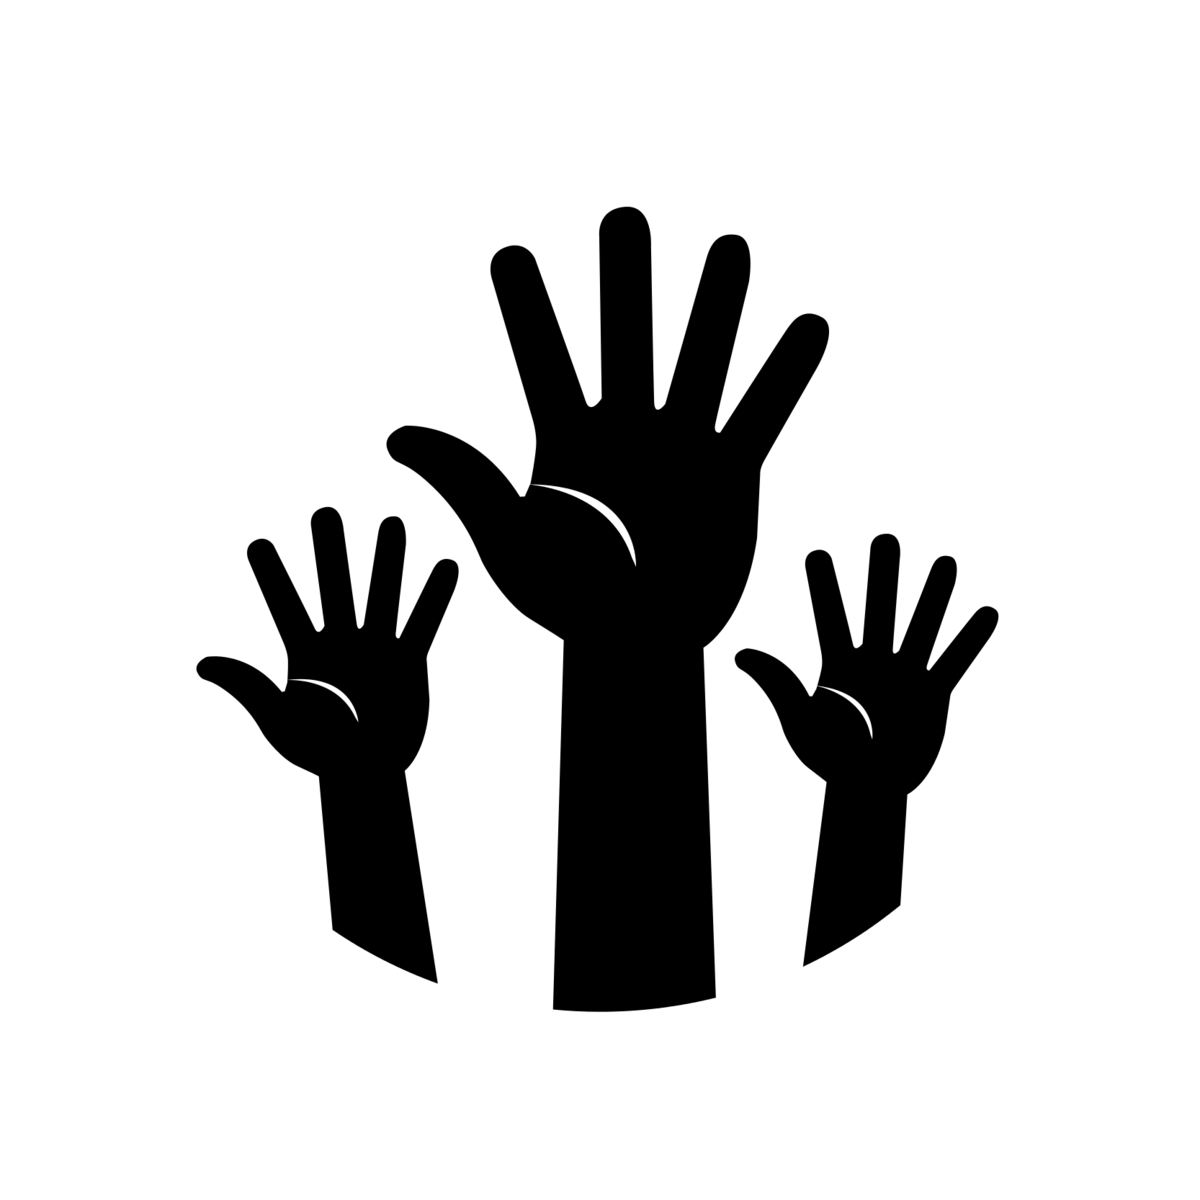
\includegraphics[scale=.03]{images/hands.png}
\alert{Design decisions?}:\\
\pause recombination (e.g., how many split points), parent selection

\end{frame}
%----------------------------------------------------------------------
%----------------------------------------------------------------------
\begin{frame}[c]{Genetic Algorithms: Selection and Evaluation}

\begin{block}{Design decisions:}
\begin{itemize}
  \item Evaluate all individuals and select best ones (also called tournament)
  \begin{itemize}
    \item how many to select?
  \end{itemize}
  \pause
  \item Evaluate only half of population (competitive half) and use selection on these
  \begin{itemize}
    \item Stronger diversification; less risk of local optima
    \item How to split population?
  \end{itemize}
  \pause
  \item Remove individuals only if they have certain age\\ (survived $n$ iterations)
  \begin{itemize}
    \item Stronger diversification; slower convergence to local optima
    \item $n$?
  \end{itemize}
  \pause
  \item \ldots
\end{itemize}
\end{block}

$\leadsto$ Again many design choices

\end{frame}
%----------------------------------------------------------------------
%----------------------------------------------------------------------
\begin{frame}[c]{}

\centering
\huge
Machine Learning Algorithms

\end{frame}
%----------------------------------------------------------------------
\begin{frame}[c]{k-Nearest Neighbor}

\includegraphics[width=0.8\textwidth]{images/kNN}

\end{frame}
%-----------------------------------------------------------------------
%----------------------------------------------------------------------
\begin{frame}[c]{k-Nearest Neighbor}

\begin{block}{Training}
Nothing to do (na\"ive implementation)
\end{block}

\bigskip

\begin{block}{Predict (Classification)}
\begin{enumerate}
  \item Determine the $k$ nearest neighbors in feature space $\mathcal{X}$
  \item Return the most often used class of the neighbors
\end{enumerate}
\end{block}

\pause
\begin{block}{Predict (Regression)}
\begin{enumerate}
  \item Determine the $k$ nearest neighbors in feature space $\mathcal{X}$
  \item Return the average value of the neighbors
\end{enumerate}
\end{block}

\end{frame}
%-----------------------------------------------------------------------
%----------------------------------------------------------------------
\begin{frame}[c]{Design Decisions in k-Nearest Neighbor}

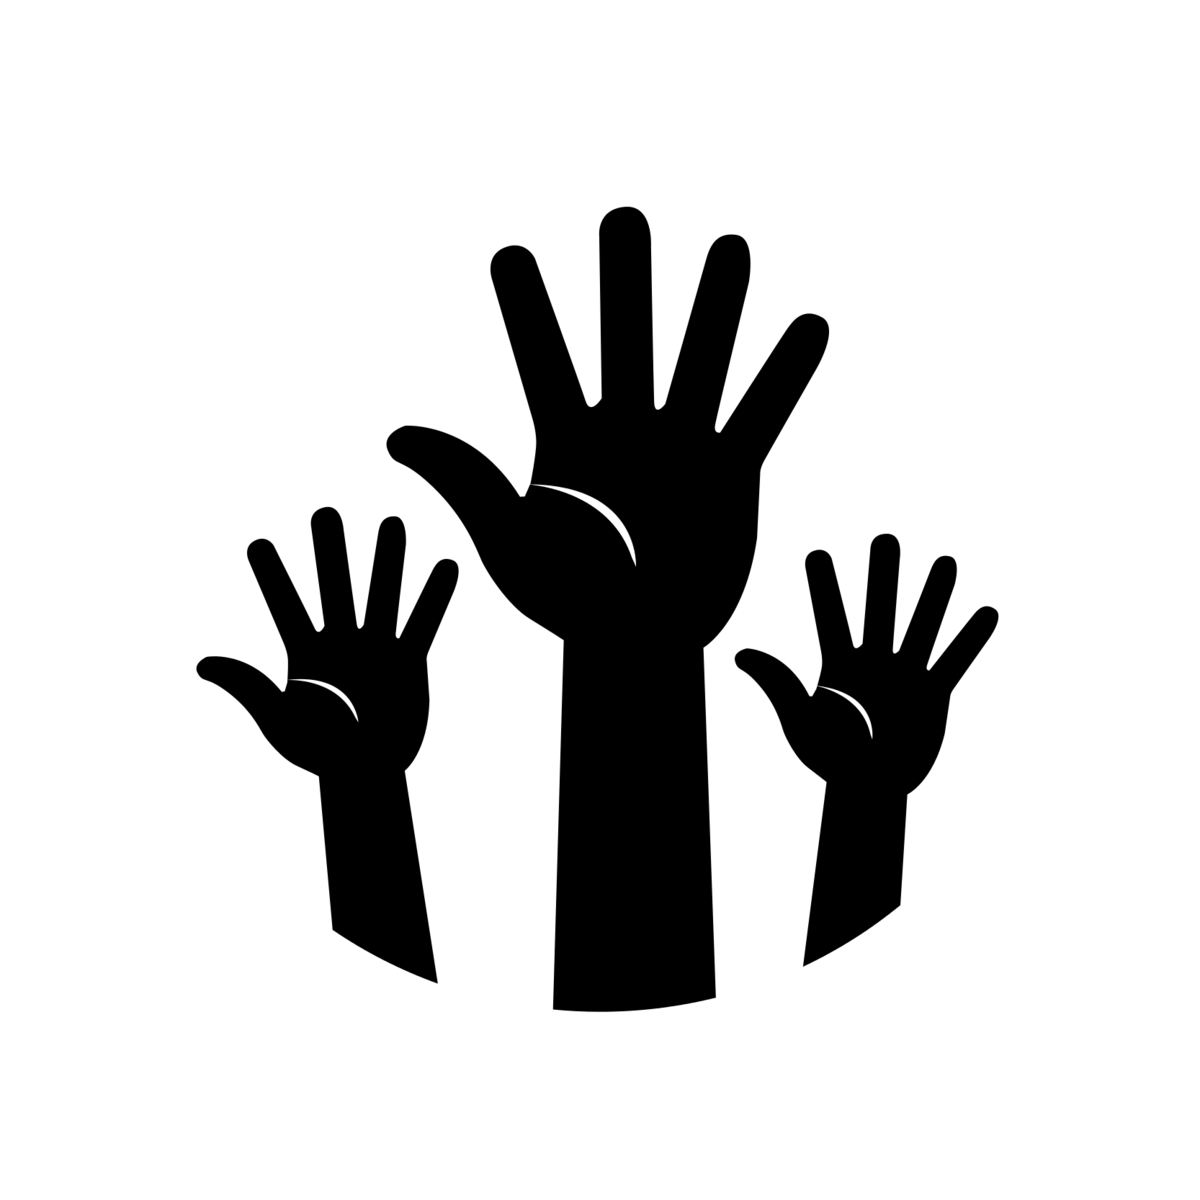
\includegraphics[scale=0.05]{images/hands}
\pause

\begin{itemize}
  \item $k$: size of neighborhood
  \item distance metric (e.g., euclidean or manhattan)
  \item (search algorithm to determine neighbors)
\end{itemize}

\end{frame}
%-----------------------------------------------------------------------
%----------------------------------------------------------------------
\begin{frame}[c]{Tuning of $k$}

\centering
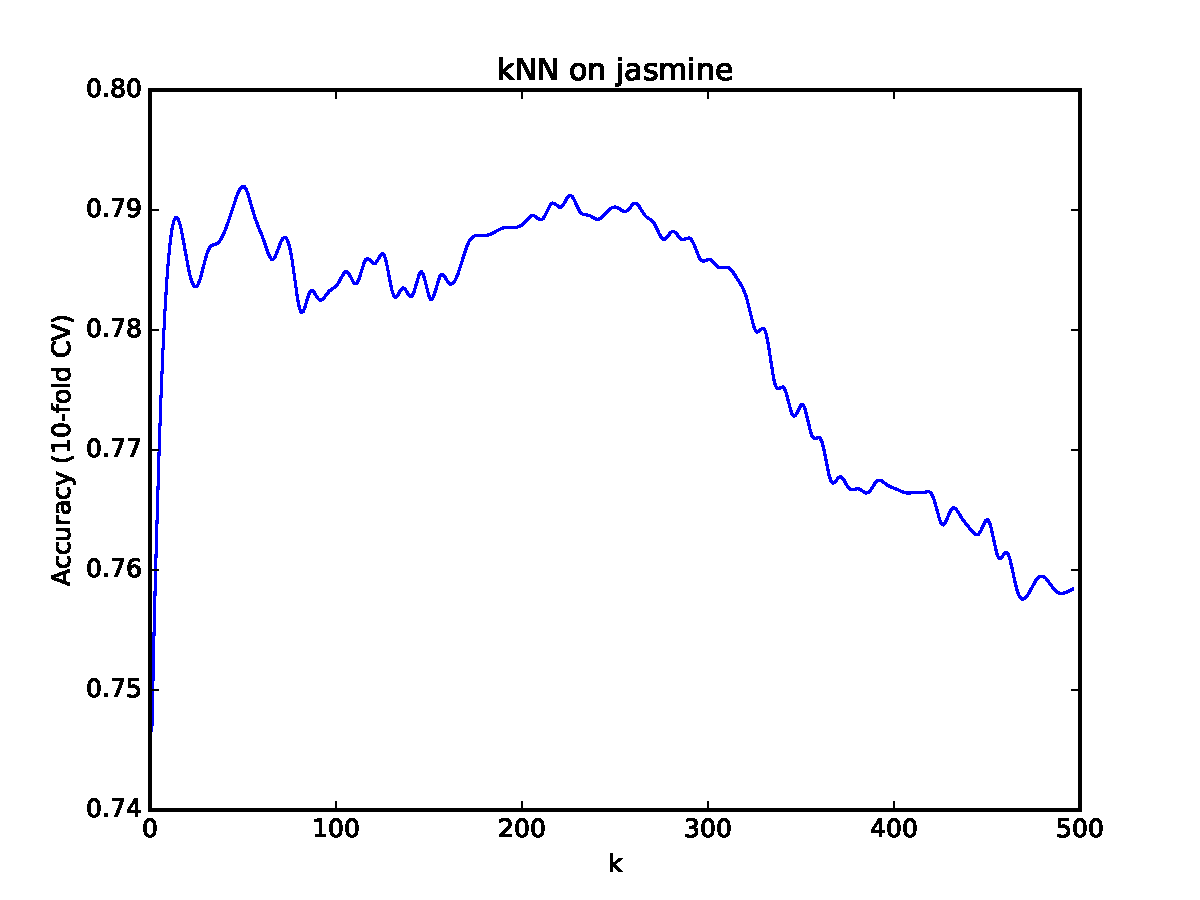
\includegraphics[scale=.5]{images/kNN-jasmine}

\end{frame}
%-----------------------------------------------------------------------
%----------------------------------------------------------------------
\begin{frame}[c]{Decision Trees}

\begin{itemize}
  \item One of the most basic ML algorithms
\end{itemize}

\centering
\includegraphics[width=0.7\textwidth]{images/iris_tree}

(source: scikit-learn)
\end{frame}
%-----------------------------------------------------------------------
%----------------------------------------------------------------------
\begin{frame}[c]{Regression Trees}

\begin{itemize}
  \item Same kind of splits, but with continuous values in leafs\\ (instead of classes)
\end{itemize}

\centering
\includegraphics[width=0.7\textwidth]{images/regression_tree_pred.png}

(source: scikit-learn)
\end{frame}
%-----------------------------------------------------------------------
%----------------------------------------------------------------------
\begin{frame}[c]{Build Decision Tree}

\begin{algorithm}[H]
\Input{$D = \{(\vec{x}^{(i)}, y^{(i)})\}_{i\in \{1\ldots|D|\}}$, attributes A}
\BlankLine
\If{all $y^{(i)}$ have the same class} {
	  \Return{Leaf with class $y$}
}
\pause
\If{attributes $=$ $\emptyset$}{
	\Return{Leaf with most frequent class}
}
\pause
let $a \in A$ be the \emph{best attribute};\\ 
\For{all values $v$ of $a$ in $D$}{
	Create edge with  constraint $a = v$;\\
	BuildTree($\{ (\vec{x}^{(i)}, y^{(i)}) \in D | \vec{x}^{(i)}.a = v\}$, $A - \{a\}$);
}
	
\Return{current node}
\caption{\texttt{BuildTree()} with categorical attributes}
\end{algorithm}

\footnotesize
\pause
Note: ``best attribute'' determined by a loss function\\ (e.g., RMSE for regression problems)\\
\pause
Note(2): loss function can be weighted by sample weights\\ (e.g., can be used for cost-sensitive algorithm selection)

\end{frame}
%-----------------------------------------------------------------------
%----------------------------------------------------------------------
\begin{frame}[c]{Design Decisions in Decision/Regression Trees?}

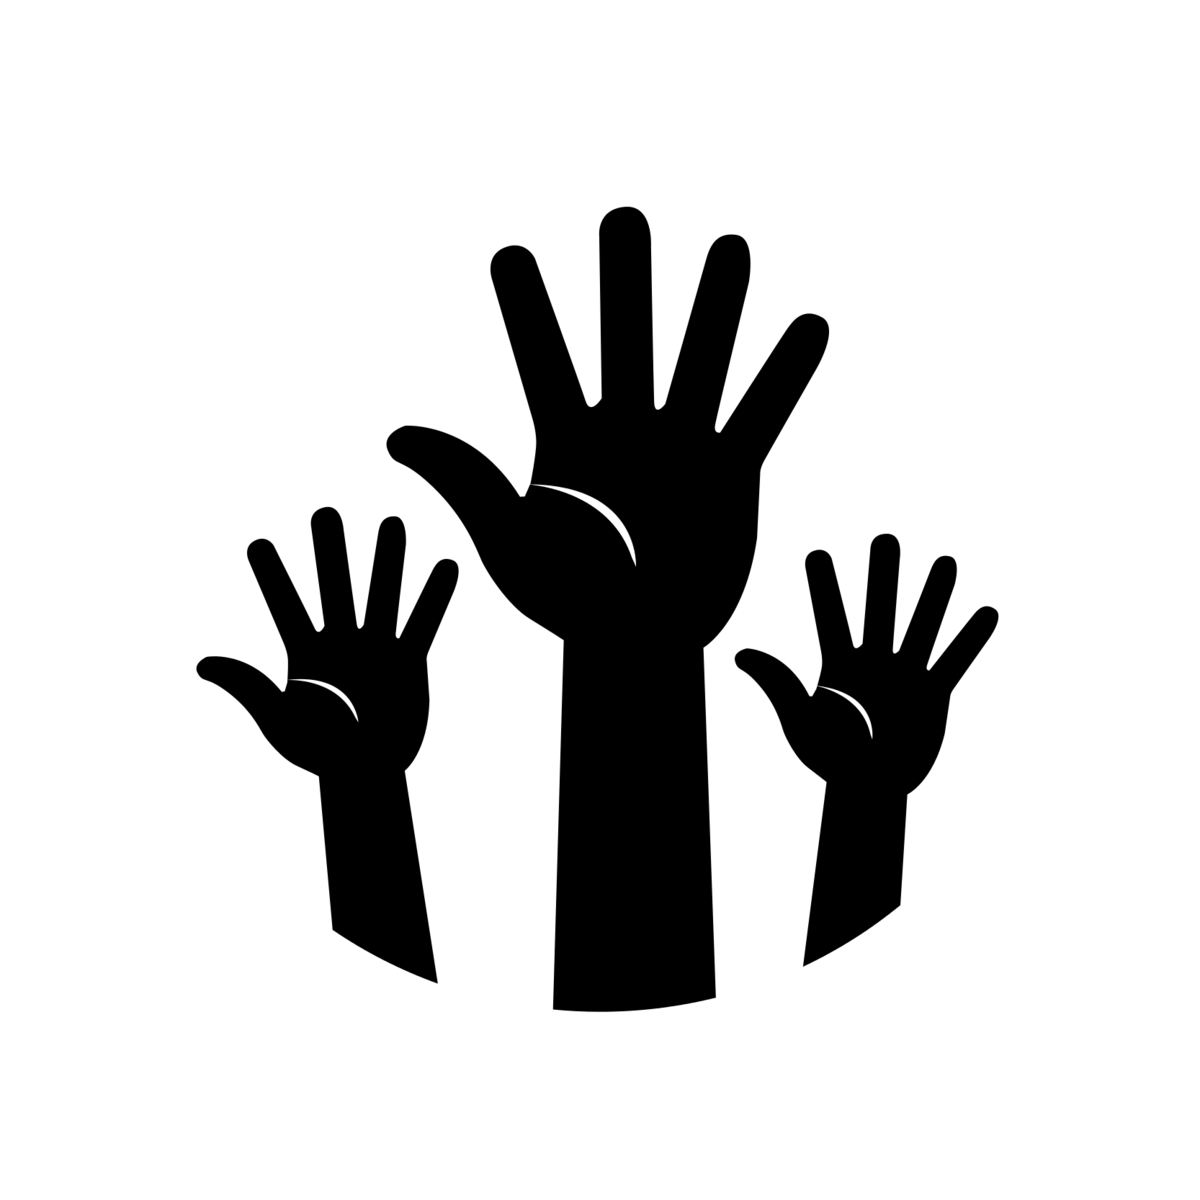
\includegraphics[scale=0.05]{images/hands}
\pause

\begin{itemize}
  \item splitting criterion (Gini, entropy, mse, \ldots)
  \item max depth
  \item min samples to split
  \item min samples in leaf
  \item max leaf nodes
  \item minimal impurity 
\end{itemize}

\end{frame}
%-----------------------------------------------------------------------
%----------------------------------------------------------------------
\begin{frame}[c]{Random Forest (Regression)}

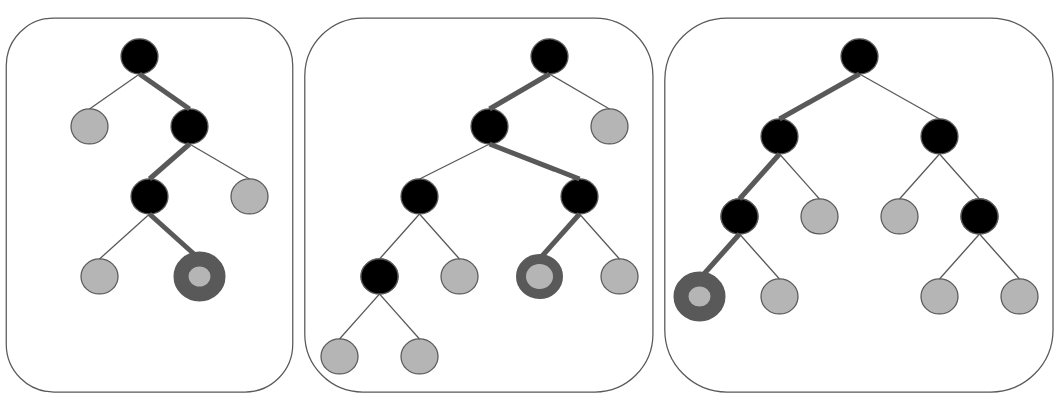
\includegraphics[width=0.9\textwidth]{images/random_forest_pic}

\begin{itemize}
  \item train several trees
  \item subsample observations and features in each tree
  \pause
  \item Prediction: average across tree predictions
  \pause
  \item Uncertainty: stdev across tree predictions
\end{itemize}

\end{frame}
%-----------------------------------------------------------------------
%----------------------------------------------------------------------
\begin{frame}[c]{Design Decisions in Random Forest}

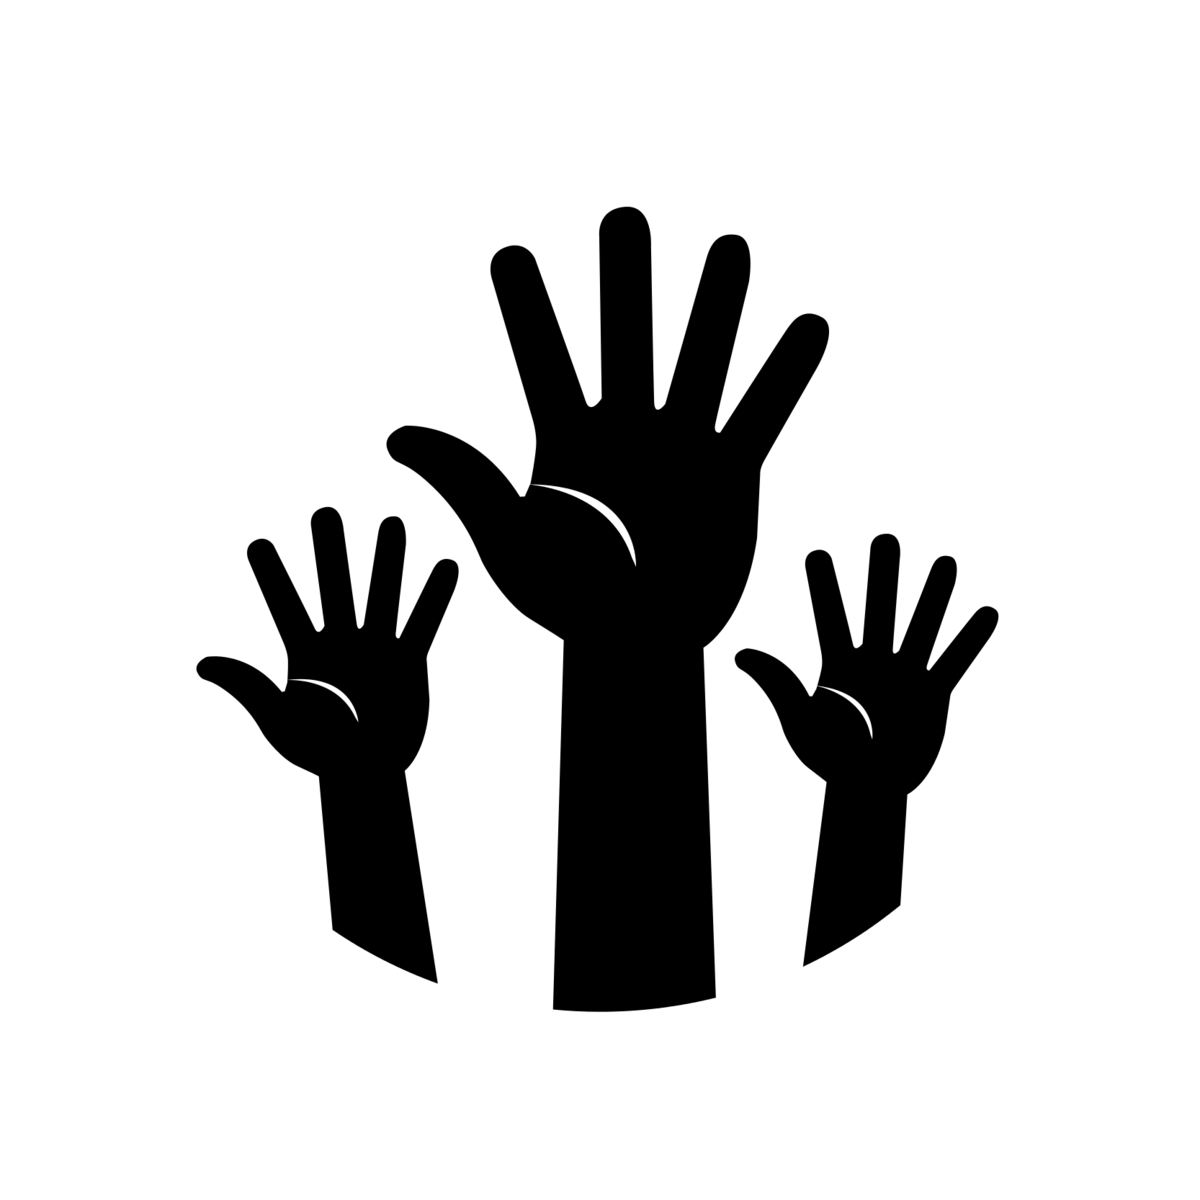
\includegraphics[scale=0.05]{images/hands}
\pause

\begin{itemize}
  \item same as for decision/regression trees
  \item aggregation strategy
  \item use of bootstrapping for sampling observations
  \item subsampling strength of observations
  \item subsampling strength of features
\end{itemize}

\end{frame}
%-----------------------------------------------------------------------
%----------------------------------------------------------------------
\begin{frame}[c]{Deep Neural Network}

\begin{itemize}
  \item most famous ML algorithm these days
  \item each layer of neurons applies a linear transformation\\
   and a non-linear activation function  $g$ on top 
\end{itemize}

\begin{eqnarray}
z_i = \vec{W}_i\vec{h_i} + \vec{b}_i\\
h_{i+1} = g(z_i)
\end{eqnarray}



\centering
\includegraphics[width=0.8\textwidth]{images/dnn_pic}

\begin{itemize}
  \item last neuron can use a softmax for $g$ (classification problem)
\end{itemize}

\end{frame}
%-----------------------------------------------------------------------
%----------------------------------------------------------------------
\begin{frame}[c]{Training of Deep Neural Network}

\begin{block}{Loss function}
\begin{itemize}
  \item Optimal weights are defined by a loss function
  \item Example of squared error (for regression)
\end{itemize}

\begin{equation}
L(\vec{W}) = \frac{1}{2} \sum_{n=1}^N \left( \hat{y}(\vec{x}_n, \vec{W}) - y_n  \right)
\end{equation}
\end{block}

\pause

\begin{block}{Optimization of loss function}
\begin{itemize}
  \item typically, we use stochastic gradient descent (SGD)\\
  (or variants of SGD)
  \item chain rule over layers to use it efficiently for deep learning
  \item Iteratively update weights (on batches of samples):
\end{itemize}

\begin{equation}
\vec{W} = \vec{W} - \eta \nabla L(\vec{W})
\end{equation}

\end{block}

\end{frame}
%-----------------------------------------------------------------------
%----------------------------------------------------------------------
\begin{frame}[c]{Design Decisions in Deep Neural Network}

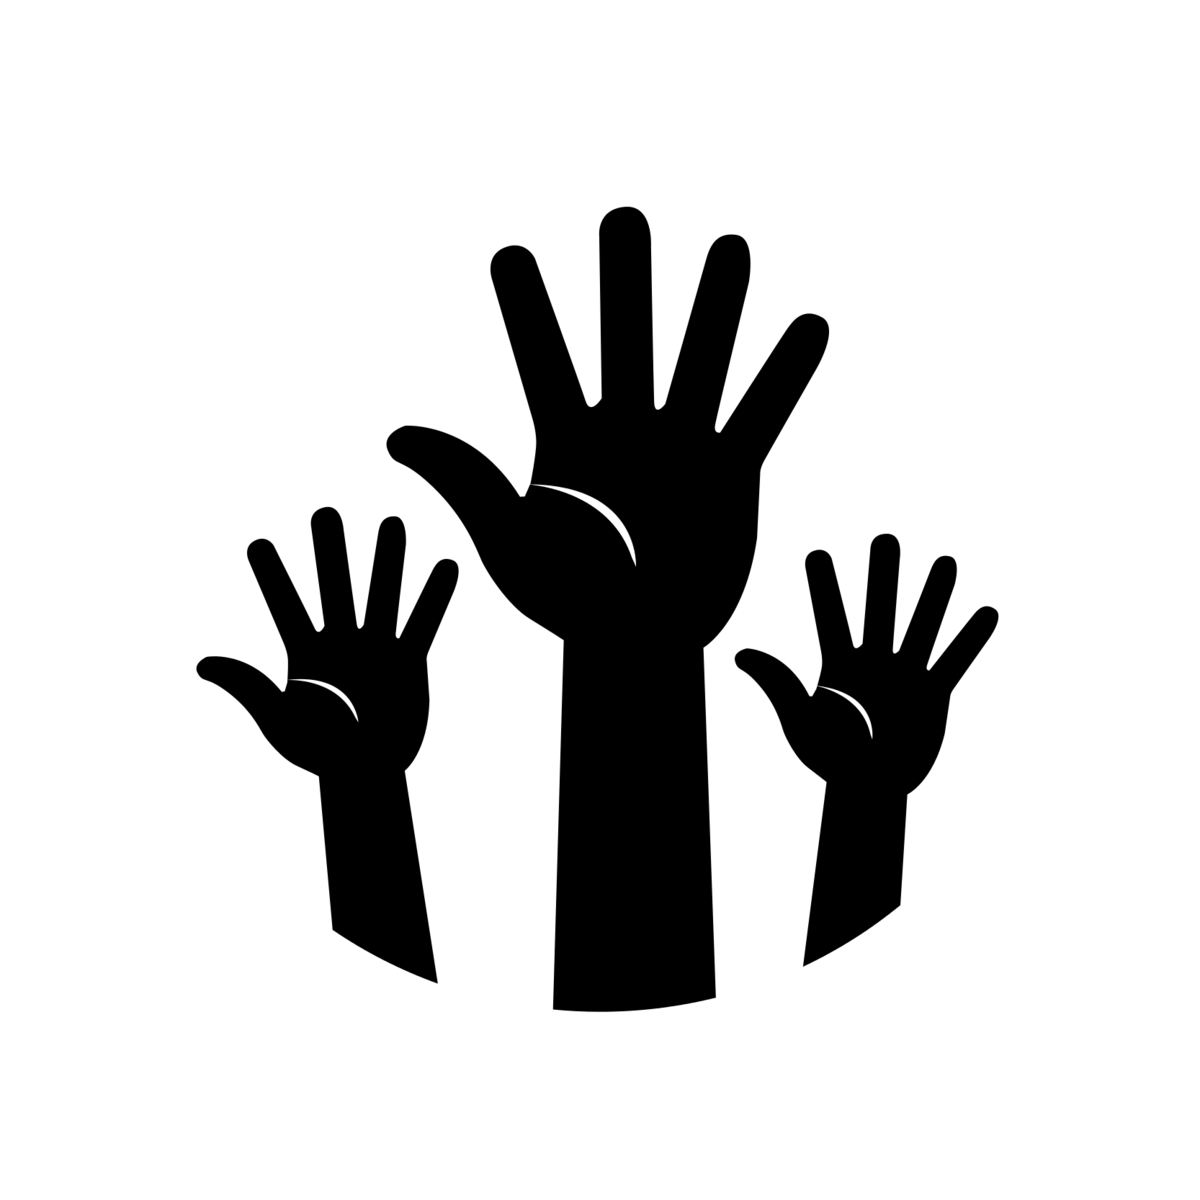
\includegraphics[scale=0.05]{images/hands}

\end{frame}
%-----------------------------------------------------------------------
\begin{frame}[c]{Summary: Learning Goals}

What have we learned today?

\begin{enumerate}
  \item Recap: Optimization algorithms
  \begin{itemize}
    \item Stochastic local search (SLS)
    \item Evolutionary algorithms
  \end{itemize}
  \item Recap: Machine learning algorithms
  \begin{itemize}
    \item kNN, tree-based algorithms, neural networks
  \end{itemize}
  \item What are typical decisions in algorithm design?
\end{enumerate}

\end{frame}
%-----------------------------------------------------------------------